\documentclass[11pt]{article}

\usepackage[T1]{fontenc}
\usepackage{lmodern}
\usepackage{amsmath,amssymb,amsthm,mathtools}
\usepackage[a4paper,margin=2.1cm]{geometry}
\usepackage{booktabs}
\usepackage{array}
\usepackage{graphicx}
\usepackage{enumitem}
\usepackage{microtype}
\usepackage{xcolor}
\usepackage[colorlinks=true,linkcolor=blue!50!black,citecolor=blue!50!black,urlcolor=blue!50!black]{hyperref}

\theoremstyle{plain}
\newtheorem{theorem}{Theorem}
\newtheorem{lemma}{Lemma}
\newtheorem{proposition}{Proposition}
\newtheorem{corollary}{Corollary}
\theoremstyle{definition}
\newtheorem{definition}{Definition}
\newtheorem{assumption}{Assumption}
\theoremstyle{remark}
\newtheorem{remark}{Remark}

\newcommand{\F}{\mathbb{F}_2}
\newcommand{\Prob}{\mathbb{P}}
\newcommand{\E}{\mathbb{E}}
\newcommand{\pL}{p_{\mathrm{L}}}
\newcommand{\pM}{p_{\mathrm{L}}^{\mathrm{MWPM}}}
\newcommand{\err}{\varepsilon^{\star}}
\newcommand{\Go}{G_{\mathrm{o}}}
\newcommand{\Co}{C_{\mathrm{o}}}
\newcommand{\cC}{\mathcal{C}}
\newcommand{\tw}{\tilde w}
\newcommand{\hw}{\hat w}
\newcommand{\td}{\tilde d}
\newcommand{\hd}{\hat d}
\newcommand{\one}{\mathbf 1}
\newcommand{\tsc}[1]{\texttt{#1}}
\let\oldunderscore\_
\renewcommand{\_}{\oldunderscore\allowbreak}
\newcommand{\sla}{/\allowbreak}
\setlength{\emergencystretch}{2em}

\title{Computable rigorous logical-error bounds for matching decoders on detector error models}
\author{[Author]\\ \small [Affiliation]}
\date{}

\begin{document}
\maketitle

\begin{abstract}
\noindent
Logical error rates of surface-code memories are usually reported as sampled estimates, and their suppression with distance as a fitted factor $\Lambda$. We give upper bounds on the per-shot logical failure probability of minimum-weight matching that are proved and can be computed on a given detector error model. The basic bound is a Peierls argument on the part of the matching graph that carries the logical observable: after re-decomposing the faults so that each one acts on a single edge, a decoder failure leaves a cycle that is at least half in error, and the sum over such cycles is bounded by a non-backtracking walk sum, evaluated by one sparse linear solve that also certifies its convergence. Two refinements use minimality of the correction more fully: every correction run on the failure cycle is a shortest path, and the total weight of the correction runs is at most the total distance bridged by the error runs. The bounds account for the integer weight rounding of pymatching and also bound the maximum-likelihood failure probability. For stim's rotated memory circuit under uniform circuit noise at $p=10^{-3}$ the sharpest bound is $6.3\times10^{-3}$, $2.0\times10^{-3}$ and $4.8\times10^{-4}$ at $d=3,5,7$, which is $8$--$26$ times the sampled pymatching rate; under assumptions on the translation structure of the circuit, checked numerically for $d\le15$, the failure probability decays at a rate corresponding to $\Lambda\ge3.97$ for every $d$, against a sampled $\Lambda\approx6$--$7$. On Google's published hardware error models the bounds are finite at the fitted noise for Willow at $d=3$ and $5$, but at $d=5$ their value exceeds $1$, and at $d=7$ the noise would have to be about $20\%$ lower for the bound to be finite. A variant takes the edge probabilities from the data's own detection statistics; it is non-vacuous only for one-round experiments at $d\le5$, and the independence assumption it needs fails in part of the data. The bounds are implemented in the open-source package \tsc{lcd-qec}.
\end{abstract}

\section{Introduction}\label{sec:intro}

Experiments on surface-code memories now report logical error rates that decrease with the code distance~\cite{Google21,Google22,Google24}. The quantities reported are estimates: the logical error rate at a given distance is a sampled frequency with a confidence interval, and the suppression factor $\Lambda$ between consecutive distances is a fit. Extrapolations to larger distances rest on that fit and on the assumption that the noise does not change its character. The same is true in simulation: the logical failure probability of a decoder on a detector error model is estimated by Monte Carlo sampling, with rare-event methods~\cite{BV,Mayer} or with closed-form approximations~\cite{Regev} when it is small.

This paper asks for upper bounds that are \emph{proved}: for a given detector error model and a given matching decoder, a number $B$ with $\pM\le B$, where $\pM$ is the per-shot probability that the decoder predicts the wrong value of the logical observable. Since maximum-likelihood decoding minimizes the failure probability, the same number bounds the maximum-likelihood failure probability $\err$. Path-counting (Peierls) arguments give such bounds for matching at code capacity~\cite{DKLP} and prove a threshold for matching under circuit-level noise~\cite{Fowler}, but their constants are far from the numerical values. Our aim is a bound whose constants are computed on the actual graph, so that it can be compared with simulation and with hardware models.

\paragraph{What is proved.}
For a detector error model whose observable part is a \emph{balanced} graph (Definition~\ref{def:obs-graph}), we prove three upper bounds on $\pM$:
\begin{itemize}[leftmargin=*,itemsep=2pt]
\item Theorem~\ref{thm:basic}: a Peierls bound written as a sum over odd cycles through the boundary vertex, bounded by a non-backtracking walk sum. The faults are re-decomposed so that every fault acts on one edge of the observable graph; this makes the edges independent, which is what the Peierls argument needs. The bound accounts for pymatching's conversion of weights to integers.
\item Theorem~\ref{thm:geodesic}: a refinement that uses the fact that every run of correction edges on the failure cycle is a shortest path.
\item Theorem~\ref{thm:gap}: a refinement that uses minimality for all runs at once (a ``gap lemma''), which moves the Chernoff factor from the error runs to the distances they bridge.
\end{itemize}
For stim's rotated memory circuit we also prove bounds that hold for every distance (Propositions~\ref{prop:lattice} and~\ref{prop:lattice-gap}). Their proofs are complete for $5\le d\le15$, where their hypotheses are checked by computer; for $d>15$ they are conditional on those hypotheses, which concern the translation structure of the generated circuit. Finally, Proposition~\ref{prop:data-cert} turns the two-point detection statistics of an experiment into simultaneous confidence limits on the edge probabilities and hence into a bound on $\pM$ that holds with a stated probability over the data, under an independence assumption.

\paragraph{What is computed, and how tight it is.}
Table~\ref{tab:stim} and Figure~\ref{fig:bounds} compare the bounds with sampled pymatching failure rates for stim's rotated memory circuit with $d$ rounds. At $p=10^{-3}$ the sharpest bound is $8$, $16$ and $26$ times the sampled rate at $d=3,5,7$, and at $p=3\times10^{-3}$ it is $6$, $18$ and $69$ times. The basic bound is $38$--$240$ times the sampled rate at $p=10^{-3}$. The every-$d$ statements give a certified suppression factor $\Lambda^\ast\ge3.97$ at $p=10^{-3}$, against a sampled $\Lambda\approx6$--$7$. The bound becomes infinite (the walk sum diverges) above $p\approx3.6\times10^{-3}$ at $d=9$, well below the circuit-level threshold of matching.

\paragraph{Where it fails.}
We state the limitations here and return to them in Section~\ref{sec:limits}. (i) The bounds are loose by one to two orders of magnitude, and the looseness grows with $d$ and $p$. (ii) On Google's published hardware models~\cite{Google22,Google24}, evaluated at the data-fitted noise, the sharpest bound is finite for Willow at $d=3$ and $d=5$, but at $d=5$ its value lies between $2.2$ and $10.9$, so it says nothing useful; at $d=7$ it is finite only if all fault probabilities are multiplied by $0.79$ or less. For Sycamore it is finite at $d=3$ and not at $d=5$. (iii) The certified $\Lambda^\ast$ refers to stim's uniform circuit noise, not to hardware. (iv) The data certificate (Section~\ref{sec:data}) is non-vacuous only for one-round experiments at $d\le5$; its independence assumption is violated in part of the hardware data, which we test and report. (v) All numbers are computed in floating point, without interval arithmetic. (vi) The hypotheses of the every-$d$ statements are checked only for $d\le15$. (vii) The bounds concern minimum-weight matching with the decoder's own weights; correlated matching~\cite{FowlerCorr}, belief matching~\cite{BeliefMatching} and neural decoders are not covered.

\paragraph{Contributions.}
To our knowledge, the following are new: (1) a Peierls bound for matching that applies to any detector error model with a balanced observable graph, made rigorous at circuit level by re-decomposition and exclusivity, including pymatching's weight rounding (Theorem~\ref{thm:basic}); (2) the geodesic and gap refinements and their computable forms (Theorems~\ref{thm:geodesic} and~\ref{thm:gap}); (3) every-$d$ bounds and certified suppression exponents for stim's rotated memory circuit (Propositions~\ref{prop:lattice} and~\ref{prop:lattice-gap}); (4) a confidence-level certificate from detection statistics (Proposition~\ref{prop:data-cert}); (5) an evaluation on published hardware models in terms of a certifiability margin; and (6) an open-source implementation, \tsc{lcd-qec}, with a command-line tool and an interface to sinter. Related work is discussed in Section~\ref{sec:related}.

\section{Setting}\label{sec:setting}

\subsection{Detector error models and matching}

A detector error model consists of independent fault mechanisms $m$, each firing with probability $p_m\in[0,\tfrac12]$; a firing mechanism flips the detectors in a set $D_m$ and the logical observable by $L_m\in\F$. We treat one observable; several observables are handled by a union bound (Section~\ref{sec:software}). The syndrome $s$ is the set of flipped detectors.

A \emph{decoding graph} $G$ has as vertices the detectors and one boundary vertex $b$. Every edge $e$ joins two detectors, or a detector and $b$, and carries an observable flag $o_e\in\F$ and a weight $w_e\ge0$. For an edge set $F$ we write $\partial F$ for the set of detectors of odd degree in $F$ (the boundary vertex is not counted), $o(F)=\sum_{e\in F}o_e$ and $w(F)=\sum_{e\in F}w_e$. A \emph{matching decoder} outputs, for the syndrome $s$, an edge set $C$ of $G$ of minimum weight with $\partial C=s$ (ties broken arbitrarily), and predicts the observable flip $o(C)$. We allow the decoder to minimize weights $\tw_e$ that differ from the $w_e$ used in the analysis; this is needed because pymatching~\cite{SB} converts its weights to integers (Theorem~\ref{thm:basic}(d)).

Let $\pM$ be the probability that the decoder's prediction differs from the actual flip $\sum_m f_mL_m$, where $f_m$ indicates that $m$ fires. Let $\err$ be the smallest failure probability of any function of the syndrome, that is, the failure probability of the maximum-likelihood (maximum a posteriori) decoder of the logical class.

\begin{lemma}[Maximum likelihood is the Bayes decoder]\label{lem:bayes}
For every decoder, $\err\le$ its failure probability; in particular $\err\le\pM$.
\end{lemma}
\begin{proof}
The failure probability of a decoder $g$ is $\sum_s\Prob[s]\,\Prob[\ell\ne g(s)\mid s]$, where $\ell$ is the actual flip; it is minimized term by term by choosing $g(s)$ to maximize $\Prob[\ell\mid s]$.
\end{proof}

\noindent For stabilizer codes the identification of maximum-likelihood decoding with the optimal guess of the logical class is standard~\cite{DKLP,IyerPoulin,Pryadko}. All upper bounds below are bounds on $\pM$ and therefore on $\err$; they cannot be falsified by data from other decoders, only by failure rates of the same matching decoder above them.

\subsection{The observable graph}

\begin{definition}[Observable graph, decompositions, balance, exclusivity]\label{def:obs-graph}
The \emph{observable graph} $\Go$ consists of the connected components of $G-b$ that contain an edge with $o_e=1$, together with their edges to $b$. We assume that parallel edges carry the same flag and are merged, so that at most one edge joins two vertices.
A \emph{graph decomposition} assigns to every mechanism $m$ an edge set $\Gamma(m)$ of $\Go$ with $\partial\Gamma(m)=D_m\cap V(\Go)$ and $o(\Gamma(m))=L_m$.
$\Go$ is \emph{balanced} if every cycle of $\Go-b$ has $o=0$. Then there is a function $\phi$ on the detectors of $\Go$ with $o_{xy}=\phi(x)+\phi(y)$ on every edge of $\Go-b$ (one $\phi$ per component), and every detector $u$ with an edge to $b$ has a \emph{side} $\sigma(u)=o_{ub}+\phi(u)\in\F$.
A mechanism is \emph{exclusive} if no simple cycle $\gamma$ with $o(\gamma)=1$ contains two edges of $\Gamma(m)$; for example, if $|\Gamma(m)|=1$, or if all edges of $\Gamma(m)$ go to $b$ from detectors of the same side.
\end{definition}

The function $\phi$ exists because, in a balanced component, the parity of $o$ along a path between two detectors does not depend on the path. Stim's \tsc{decompose\_errors=True} provides a graph decomposition, with $G$ the graph of its components, provided that no two components with the same detectors carry different flags (\emph{flag consistency}). Any other decomposition may be used. In particular, if the detectors of a mechanism in $\Go$ are those of one edge $e$ with $o_e=L_m$, we may set $\Gamma(m)=\{e\}$; we call this \emph{re-decomposition}. It matters: at circuit level stim splits some faults into two edges to the boundary, and two such edges can lie on one odd cycle, so the edges of $\Go$ are not independent. After re-decomposition, every mechanism of the circuits studied in Section~\ref{sec:numerics} has exactly one edge in $\Go$.

For an edge $e$ of $\Go$ let
\[
q_e=\tfrac12\Big(1-\prod_{m\ \text{exclusive},\ e\in\Gamma(m)}(1-2p_m)\Big),
\]
the probability that an odd number of the exclusive mechanisms on $e$ fire. Let $\cC$ be the set of simple cycles of $\Go$ through $b$ whose two edges at $b$ end at detectors of different sides.

\begin{lemma}[Failure leaves a heavy odd cycle]\label{lem:cycle}
Let $X=\bigoplus_{m:\,f_m=1}\Gamma(m)$ (symmetric difference) and $\Co=C\cap E(\Go)$, where $C$ minimizes $\tw$. If $\Go$ is balanced and the decoder fails, there is $\gamma\in\cC$ with $\gamma\subseteq X\oplus\Co$, $\gamma\cap X=\gamma\setminus\Co$ and $\tw(\gamma\cap\Co)\le\tw(\gamma\cap X)$.
\end{lemma}
\begin{proof}
$\partial X=s\cap V(\Go)$, and $o(X)=\sum_mf_mL_m$ is the actual flip. The boundary vertex imposes no constraint, so the minimization splits over the components of $G-b$; hence $\Co$ is a minimum-$\tw$ edge set of $\Go$ with $\partial\Co=s\cap V(\Go)$, and the other edges of $C$ have $o_e=0$. So the decoder fails iff $o(X\oplus\Co)=1$. $Y=X\oplus\Co$ has even degree at every detector, hence also at $b$, so it is an edge-disjoint union of simple cycles; on failure one of them, $\gamma$, has $o(\gamma)=1$. Since $\Co\oplus\gamma$ has the same boundary as $\Co$, minimality gives $\tw(\gamma\cap\Co)\le\tw(\gamma\setminus\Co)$, and $\gamma\setminus\Co=\gamma\cap X$ because every edge of $\gamma\subseteq Y$ lies in exactly one of $X$ and $\Co$. By balance $\gamma$ passes through $b$; if its edges at $b$ are $ub$ and $vb$, then $1=o(\gamma)=o_{ub}+\phi(u)+\phi(v)+o_{vb}=\sigma(u)+\sigma(v)$, so $\gamma\in\cC$.
\end{proof}

\section{The basic bound}\label{sec:basic}

\begin{theorem}[Circuit-level Peierls bound for matching]\label{thm:basic}
Let $\Go$ be balanced, let $\Gamma$ be a graph decomposition, and let the decoder minimize weights $\tw_e$ with $|\tw_e/s-w_e|\le\delta$ on every edge of $\Go$, for some $s>0$ and $\delta\ge0$ ($\delta=0$ if it minimizes $w$). For a non-exclusive mechanism $m$ put $k_m=|\Gamma(m)|$. For $\lambda\ge0$ let $a_e=e^{2\lambda w_e}$ and
\[
\beta_e(\lambda)=e^{\lambda(\delta-w_e)}\,(1-q_e+q_ea_e)\prod_{m\ \text{not exclusive},\ e\in\Gamma(m)}\big(1+p_m^{1/k_m}(a_e-1)\big).
\]
\begin{enumerate}[label=(\alph*),leftmargin=*]
\item For every $\lambda\ge0$, $\ \pM\le\sum_{\gamma\in\cC}\prod_{e\in\gamma}\beta_e(\lambda)$.
\item Let $B$ be the non-backtracking matrix of $\Go-b$ on directed edges, $B_{(x\to y),(y\to z)}=\beta_{yz}$ for $z\ne x$ and $0$ otherwise. Put $\mathrm{start}_{(u\to y)}=\beta_{ub}\beta_{uy}$ if $u$ has an edge to $b$ and $\sigma(u)=0$, and $\mathrm{end}_{(x\to v)}=\beta_{vb}$ if $v$ has an edge to $b$ and $\sigma(v)=1$, both $0$ otherwise. If the spectral radius $\rho(B)<1$, the sum in (a) is at most $\mathrm{start}^{\mathsf T}(I-B)^{-1}\mathrm{end}$.
\item $\err\le\pM$. For fixed weights, the bounds (a) and (b) are nondecreasing in every $p_m\in[0,\tfrac12]$, so they remain valid with each $p_m$ replaced by an upper limit $\bar p_m\le\tfrac12$.
\item (Pymatching.) Pymatching~2~\cite{SB} minimizes $\tw_e=2\,\mathrm{round}(\varkappa w_e)$, where $w_e$ are its floating-point weights and $\varkappa=(2^{24}-1)/\max_e|w_e|$. So the theorem applies with its own weights $w_e$, $s=2\varkappa$ and $\delta=\max_e|w_e|/(2(2^{24}-1))$.
\end{enumerate}
\end{theorem}

\begin{proof}
\emph{One cycle.} Fix $\gamma\in\cC$ and let $x_e=\one[e\in X]$. By Lemma~\ref{lem:cycle}, failure through $\gamma$ requires $\tw(\gamma\cap\Co)\le\tw(\gamma\cap X)$. Writing $\tw_e=s(w_e+\epsilon_e)$ with $|\epsilon_e|\le\delta$ gives $w(\gamma\cap\Co)-w(\gamma\cap X)\le\delta|\gamma|$, and since $\gamma$ is the disjoint union of $\gamma\cap\Co$ and $\gamma\cap X$, $w(\gamma\cap X)\ge\tfrac12w(\gamma)-\tfrac12\delta|\gamma|$. For $\lambda\ge0$ the indicator of this event is at most $\prod_{e\in\gamma}e^{\lambda(\delta-w_e)}a_e^{x_e}$ (Chernoff).
Let $y_e$ be the parity of the firing exclusive mechanisms with $e\in\Gamma(m)$. Then $x_e\le y_e+\sum f_m$, the sum over the non-exclusive $m$ with $e\in\Gamma(m)$, and $a_e\ge1$, so $a_e^{x_e}\le a_e^{y_e}\prod a_e^{f_m}$. An exclusive mechanism has at most one edge on $\gamma$, so the $y_e$, $e\in\gamma$, are functions of disjoint sets of mechanisms; they are independent of each other and of the non-exclusive mechanisms, with $\Prob[y_e=1]=q_e$. Hence
\[
\begin{multlined}
\Prob\big[\text{failure through }\gamma\big]\le\prod_{e\in\gamma}e^{\lambda(\delta-w_e)}(1-q_e+q_ea_e)\\
\times\prod_{m\ \text{not excl.}}\Big(1-p_m+p_m\prod_{e\in\gamma\cap\Gamma(m)}a_e\Big).
\end{multlined}
\]
\emph{Splitting.} If $t_i\ge0$, $r_i\in[0,1]$ and $\prod_ir_i\ge p$, then $1+p\big(\prod_i(1+t_i)-1\big)\le\prod_i(1+r_it_i)$: after expansion, the coefficient of $\prod_{i\in S}t_i$ ($S\ne\emptyset$) is $p$ on the left and $\prod_{i\in S}r_i\ge p$ on the right. With $t_e=a_e-1$ and $r_e=p_m^{1/k_m}$ for $e\in\gamma\cap\Gamma(m)$ we have $\prod r_e=p_m^{|\gamma\cap\Gamma(m)|/k_m}\ge p_m$, so the factor of $m$ is at most $\prod_{e\in\gamma\cap\Gamma(m)}(1+p_m^{1/k_m}(a_e-1))$. Altogether the probability is at most $\prod_{e\in\gamma}\beta_e(\lambda)$, and a union bound over $\cC$ (Lemma~\ref{lem:cycle}) gives (a).

\emph{Walks.} Orient $\gamma\in\cC$ from its end $u$ on side $0$: it reads $b,u=x_0,x_1,\dots,x_n=v,b$ with $n\ge1$ (at most one edge joins $u$ and $b$), and $x_0\cdots x_n$ is a simple path, hence a non-backtracking walk in $\Go-b$. Its weight $\prod_{e\in\gamma}\beta_e$ equals $\mathrm{start}_{(x_0\to x_1)}\prod_{i=1}^{n-1}B_{(x_{i-1}\to x_i),(x_i\to x_{i+1})}\,\mathrm{end}_{(x_{n-1}\to x_n)}$, and different cycles give different walks. All terms are nonnegative, so the sum in (a) is at most $\sum_{n\ge0}\mathrm{start}^{\mathsf T}B^n\mathrm{end}=\mathrm{start}^{\mathsf T}(I-B)^{-1}\mathrm{end}$ when $\rho(B)<1$.

(c) The first claim is Lemma~\ref{lem:bayes}. $1-q+qa_e$ is nondecreasing in $q$ ($a_e\ge1$), and $q_e$ is nondecreasing in each $p_m\le\tfrac12$; the factors $1+p^{1/k}(a_e-1)$ are nondecreasing in $p$; the Neumann series and $\rho(B)$ are nondecreasing in every entry of $B$. The weights are the decoder's and are held fixed.

(d) This is read off pymatching's source (version 2.4.0, files \tsc{sparse\_blossom\sla driver\sla user\_graph.h} and \tsc{user\_graph.cc}): weights are scaled by $\varkappa$, rounded to integers and doubled. Rounding moves $\varkappa w_e$ by at most $\tfrac12$, so $|\tw_e/(2\varkappa)-w_e|\le1/(2\varkappa)=\delta$.
\end{proof}

\paragraph{Evaluation.} The computation solves $(I-B)z=\one$ by a sparse LU factorization. If $z>0$, then $Bz=z-\one\le(1-1/\max_iz_i)\,z$, so $\rho(B)\le1-1/\max_iz_i<1$ by the Collatz--Wielandt bound for nonnegative matrices~\cite{HornJohnson}; the same factorization then evaluates $\mathrm{start}^{\mathsf T}(I-B)^{-1}\mathrm{end}$. If no positive solution exists, the bound is reported as infinite. Each $\beta_e(\lambda)$ is a positive combination of exponentials in $\lambda$, so the bound in (a) is log-convex in $\lambda$ and the optimization over $\lambda$ is one-dimensional; with log-likelihood weights the optimum is close to $\lambda=\tfrac12$. For the circuits of Section~\ref{sec:numerics}, $\delta\approx1.9\times10^{-7}$; the factor $e^{\lambda\delta|\gamma|}$ changes no printed digit, but all numbers include it.

\begin{remark}[Code capacity]\label{rem:cc}
At code capacity every qubit is one mechanism with one edge, and with $w_e=\ln\frac{1-q}{q}$ and $\lambda=\tfrac12$ one gets $\beta_e=2\sqrt{q(1-q)}$. Bounding the number of cycles of length $\ell$ through the boundary by $d\,3^{\ell-1}$ on the rotated surface code gives $\pM\le 2d\,\beta(3\beta)^{d-1}/(1-3\beta)$ for the two independent matching problems ($3\beta<1$), the Dennis--Kitaev--Landahl--Preskill estimate~\cite{DKLP}; erased qubits can be included as weight-$0$ edges with $\beta_e=1$. Part (b) replaces the count $d\,3^{\ell-1}$ by the exact non-backtracking walk sum on the graph.
\end{remark}

\paragraph{Bursts.} The same argument handles a simple model of bursts. Let all mechanisms be exclusive, and let \emph{burst regions} $z$ be sets of mechanisms that are activated independently, $\Prob[z\text{ active}]\le\rho_z$; an activation raises the probability of each mechanism of $z$ to an arbitrary value in $[p_m,\tfrac12]$, independently across mechanisms given the activations.

\begin{proposition}[Bursts]\label{prop:bursts}
In this model let $E(z)=\bigcup_{m\in z}\Gamma(m)$, $V_E=\max_z|E(z)|$, $\bar\rho_E=\max_e\sum_{z:\,E(z)\ni e}\rho_z$, $\kappa_e=\tfrac12e^{\lambda(\delta-w_e)}(1+a_e)/\beta_e(\lambda)\ge1$ and $\bar\kappa=\max_e\kappa_e$. Then Theorem~\ref{thm:basic}(a),(b) hold, uniformly in the burst strengths, with every $\beta_e$ replaced by $\beta_e\,\Xi$, where $\Xi=\exp\big(\bar\rho_E(\bar\kappa^{V_E}-1)/V_E\big)$.
\end{proposition}
\begin{proof}
Given the activations the mechanisms are independent. An edge not in $E(z)$ for an active $z$ keeps $q_e$; an edge hit by an active region has parity probability in $[q_e,\tfrac12]$, and $\tfrac12$ gives the largest factor $\tfrac12e^{\lambda(\delta-w_e)}(1+a_e)=\kappa_e\beta_e$. So, given the activations, failure through $\gamma$ has probability at most $\prod_{e\in\gamma}\beta_e\prod_z\bar\kappa^{k_z\one[z\text{ active}]}$ with $k_z=|\gamma\cap E(z)|\le V_E$. Averaging over the independent activations gives the factor $\prod_z(1+\rho_z(\bar\kappa^{k_z}-1))\le\exp\sum_z\rho_z(\bar\kappa^{k_z}-1)$. By convexity, $\bar\kappa^{k}-1\le k(\bar\kappa^{V_E}-1)/V_E$ for $0\le k\le V_E$, and $\sum_z\rho_zk_z\le|\gamma|\bar\rho_E$, so the factor is at most $\Xi^{|\gamma|}$. The walk bound follows as before.
\end{proof}

\noindent In particular, bursts with bounded size and rate multiply each edge factor by a constant and do not create a $d$-independent floor of the bound as long as the walk sum still converges. We do not evaluate Proposition~\ref{prop:bursts} on data in this paper.

\section{Refinements}\label{sec:refinements}

The Peierls step of Theorem~\ref{thm:basic} sums over all subsets $S=\gamma\cap X$ of an odd cycle that carry at least half its weight. Minimality of the correction restricts the complement $\gamma\setminus S$ much more. Throughout this section all mechanisms are exclusive and the decoder minimizes positive weights $\tw_e>0$; put $\hw=\tw/s$ for a fixed $s>0$ (for pymatching, $s=2\varkappa$), and let $\td$ and $\hd=\td/s$ be the corresponding graph distances in $\Go$. A \emph{run} of an edge set $F\subseteq\gamma$ is a maximal sequence of consecutive edges of $\gamma$ in $F$; it is a path of $\Go$, possibly through $b$.

\subsection{Geodesic refinement}

\begin{lemma}[Correction runs are geodesics]\label{lem:geodesic}
In the situation of Lemma~\ref{lem:cycle}, $S=\gamma\cap X\ne\emptyset$, and every run of $\gamma\setminus S=\gamma\cap\Co$ is a $\tw$-geodesic of $\Go$ between its end points.
\end{lemma}
\begin{proof}
$S\ne\emptyset$ because $\tw(\gamma\cap\Co)\le\tw(S)$ and the weights are positive. Let $\sigma$ be a run of $\gamma\cap\Co$ from $u$ to $v$ and $\sigma'$ any $u$--$v$ path of $\Go$. The edge set $\sigma\oplus\sigma'$ has even degree at every detector, so $C'=\Co\oplus\sigma\oplus\sigma'$ has the boundary of $\Co$. As $\sigma\subseteq\Co$, $\tw(C')\le\tw(\Co)-\tw(\sigma)+\tw(\sigma')$, and minimality gives $\tw(\sigma)\le\tw(\sigma')$.
\end{proof}

\begin{theorem}[Geodesic refinement]\label{thm:geodesic}
Let $\Go$ be balanced, all mechanisms exclusive and $\tw>0$. For $\lambda\ge0$ put $x_e=q_ee^{\lambda\hw_e}$ and $c_e=(1-q_e)e^{-\lambda\hw_e}$.
\begin{enumerate}[label=(\alph*),leftmargin=*]
\item $\displaystyle\pM\le\sum_{\gamma\in\cC}\ \sum_{S}\ \prod_{e\in S}x_e\prod_{e\in\gamma\setminus S}c_e$, the inner sum over the nonempty $S\subseteq\gamma$ whose complement has only $\tw$-geodesic runs.
\item (Computable form.) On the detectors of $\Go$ let $K_X(y,z)$ be the sum of $\prod x_e$ over non-backtracking walks of length $\ge1$ from $y$ to $z$ in $\Go-b$, and $K_C(y,z)$, $y\ne z$, the sum of $\prod c_e$ over paths from $y$ to $z$ in $\Go-b$ that are $\tw$-geodesics of $\Go$. Let $\sigma_i(u)=x_{ub}$ if $u$ has an edge to $b$ and $\sigma(u)=i$, and $0$ otherwise; $s_X=\sigma_0^{\mathsf T}(I+K_X)$ and $e_X=(I+K_X)\sigma_1$; and let $s_C(z)$ (resp.\ $e_C(z)$) be the sum of $\prod c_e$ over the $\tw$-geodesics of $\Go$ from $b$ to $z$ whose first edge ends on side $0$ (resp.\ $1$) and which avoid $b$ afterwards. With $M=\begin{pmatrix}0&K_C\\K_X&0\end{pmatrix}$, if $\rho(M)<1$ and the walk sums converge,
\[
\pM\le s_X\sigma_1+(s_X,\,s_C)\,(I-M)^{-1}\begin{pmatrix}e_C\\ e_X\end{pmatrix}.
\]
\item $\err\le\pM$, so (a) and (b) bound $\err$ as well.
\end{enumerate}
\end{theorem}
\begin{proof}
(a) Fix $\gamma$ and $S$. The event $\gamma\cap X=S$ is the event $S\subseteq X$, $(\gamma\setminus S)\cap X=\emptyset$. By exclusivity the indicators $\one[e\in X]$, $e\in\gamma$, are independent with probabilities $q_e$, so the event has probability $\prod_Sq_e\prod_{\gamma\setminus S}(1-q_e)$. On it, failure through $\gamma$ needs $\tw(\gamma\setminus S)\le\tw(S)$ (Lemma~\ref{lem:cycle}), whose indicator is at most $\exp\big(\lambda(\hw(S)-\hw(\gamma\setminus S))\big)$. By Lemmas~\ref{lem:cycle} and~\ref{lem:geodesic}, the union over $\gamma\in\cC$ and the admissible $S$ covers the failure event.

(b) Orient $\gamma\in\cC$ from its end on side $0$, so that it reads $b,u,\dots,v,b$, and cut it at $b$. Its edges fall into alternating maximal runs of $S$ (error runs) and of $\gamma\setminus S$ (correction runs); a run containing both edges at $b$ is cut into a first and a last piece. If $\gamma\subseteq S$, the term is that of a non-backtracking walk from $b$ ending with the edge $vb$, and these terms sum to at most $s_X\sigma_1$. Otherwise the sequence is: a first run from $b$ (an error run, counted in $s_X$, or a correction run, counted in $s_C$); interior runs avoiding $b$, alternating in type (an error run is a non-backtracking walk in $\Go-b$, counted in $K_X$; a correction run is a sub-path of a geodesic, hence a geodesic, counted in $K_C$); and a last run into $b$ of the type opposite to the preceding one (counted in $e_C$ or $e_X$, by the symmetry of geodesics and walks). Distinct pairs $(\gamma,S)$ give distinct sequences and all terms are nonnegative, so the sum in (a) is at most the sum over all alternating sequences, which is the Neumann series of $M$. Convergence is certified by a positive solution of $(I-M)z=\one$ as in Section~\ref{sec:basic}.

(c) Lemma~\ref{lem:bayes}.
\end{proof}

\noindent Since $x_e+c_e=\beta_e(\lambda)$ when $\hw=w$ and $\delta=0$, dropping the geodesic constraint in (a) recovers Theorem~\ref{thm:basic}(a) without its rounding slack; the slack is not needed here because the minimality step uses the decoder's weights directly.

\subsection{Gap refinement}

\begin{lemma}[Gap lemma]\label{lem:gap}
In the situation of Lemma~\ref{lem:cycle}, write the failure cycle $\gamma$ cyclically as alternating runs: correction runs $\sigma_1,\dots,\sigma_k$ ($k\ge0$) and error runs $\pi_1,\dots,\pi_k$, where $\pi_j$ goes from the end $z_j$ of $\sigma_j$ to the start $y_{j+1}$ of $\sigma_{j+1}$ (indices mod $k$). Then $\sum_i\tw(\sigma_i)\le\sum_j\td(z_j,y_{j+1})$.
\end{lemma}
\begin{proof}
Let $\tau_j$ be a $\tw$-geodesic from $z_j$ to $y_{j+1}$. The edge set $\Sigma=\bigoplus_i\sigma_i$ has odd degree exactly at the end points $\{y_i,z_i\}$ (counted mod $2$), and so does $T=\bigoplus_j\tau_j$, because the pairs $(z_j,y_{j+1})$ use every end point once. Hence $C'=\Co\oplus\Sigma\oplus T$ has the boundary of $\Co$. As the $\sigma_i\subseteq\Co$ are disjoint, $\tw(C')\le\tw(\Co)-\sum_i\tw(\sigma_i)+\sum_j\tw(\tau_j)$, and minimality gives the claim.
\end{proof}

\begin{theorem}[Gap refinement]\label{thm:gap}
In the setting of Theorem~\ref{thm:geodesic}, with the runs of Lemma~\ref{lem:gap}:
\begin{enumerate}[label=(\alph*),leftmargin=*]
\item For $\lambda\ge0$,
\[
\pM\le\sum_{\gamma\in\cC}\ \sum_{S}\ \prod_{e\in S}q_e\prod_{e\in\gamma\setminus S}(1-q_e)\ \exp\Big(\lambda\Big[\sum_j\hd(z_j,y_{j+1})-\sum_i\hw(\sigma_i)\Big]\Big),
\]
the inner sum over the nonempty $S\subseteq\gamma$ whose complement has only geodesic runs (for $S=\gamma$ the exponential is $1$).
\item (Computable form.) Let $\mathcal A$ be the arcs (directed edges) of $\Go-b$, $e(f)$ the edge of an arc $f$, $P=(I-B_q)^{-1}$ with $B_q$ the non-backtracking matrix on $\mathcal A$ with entries $q_{e(f')}$, and for arcs $f,l$
\[
K_X(f,l)=q_{e(f)}P_{fl}\,e^{\lambda\hd(\mathrm{tail}f,\,\mathrm{head}\,l)},\]
\[K_C(f,l)=c_{e(f)}c_{e(l)}F(\mathrm{head}f,\mathrm{tail}\,l)\,\one\big[\tw_{e(f)}+\td(\mathrm{head}f,\mathrm{tail}\,l)+\tw_{e(l)}=\td(\mathrm{tail}f,\mathrm{head}\,l)\big],
\]
with $K_C(f,f)=c_{e(f)}$ if $e(f)$ is a geodesic, $c_e=(1-q_e)e^{-\lambda\hw_e}$, and $F(u,w)$ the sum of $\prod c_e$ over the paths from $u$ to $w$ in $\Go-b$ that are geodesics of $\Go$ ($F(u,u)=1$). Let $J(l,f)=1$ if $\mathrm{head}\,l=\mathrm{tail}f$ and $\mathrm{head}f\ne\mathrm{tail}\,l$ (no reversal at a junction), and $0$ otherwise. If the spectral radius of $M=\begin{pmatrix}0&JK_C\\JK_X&0\end{pmatrix}$ is $<1$ and the walk sums converge, the sum in (a) is at most
\[
T_0+T_1+(s_X,s_C)(I-M)^{-1}\begin{pmatrix}e_X\\e_C\end{pmatrix}.
\]
Here $T_0$ is the sum of $\prod q_e$ over closed non-backtracking walks $b\to u\to\dots\to v\to b$ with $\sigma(u)=0$, $\sigma(v)=1$ (the terms with $S=\gamma$), and $s_X,s_C,e_X,e_C,T_1$ collect the first and last runs at $b$ as in Theorem~\ref{thm:geodesic}(b): a first or last run may consist of its boundary edge only, in which case no junction constraint applies, and a gap that passes through $b$ is bounded by $\hd(z,b)+\hd(b,y)$.
\item $\err\le\pM$.
\end{enumerate}
\end{theorem}
\begin{proof}
(a) As in Theorem~\ref{thm:geodesic}(a), with the indicator of Lemma~\ref{lem:gap} bounded by $\exp(\lambda[\sum_j\hd(z_j,y_{j+1})-\sum_i\hw(\sigma_i)])$; if $k=0$ the cycle lies in $X$ and no condition is used. The geodesic constraint is Lemma~\ref{lem:geodesic}.

(b) Cut $\gamma$ at $b$ and orient it from its end on side $0$. An error run $\pi$ from $z$ to $y$ contributes $\prod_{e\in\pi}q_e\,e^{\lambda\hd(z,y)}$ and a correction run contributes $\prod c_e$; a gap through $b$ is split at $b$ using $\hd(z,y)\le\hd(z,b)+\hd(b,y)$. An interior error run is a non-backtracking walk, counted in $K_X$ by its first and last arcs (the factor $P$ sums over all non-backtracking continuations). An interior correction run with first arc $f$ and last arc $l$ is a geodesic iff the three pieces add up to the distance between its end points, which is the indicator in $K_C$. Consecutive runs of a simple cycle meet at a vertex, and the second does not start with the reverse of the last arc of the first; this is the constraint $J$. Distinct pairs $(\gamma,S)$ give distinct sequences, all terms are nonnegative, and the sum over all sequences is the Neumann series of $M$, whose convergence is certified as before.

(c) Lemma~\ref{lem:bayes}.
\end{proof}

\noindent The arc-level form costs dense matrices of size $|\mathcal A|$; the implementation evaluates Theorems~\ref{thm:geodesic} and~\ref{thm:gap} only for models with at most $1000$ detectors.

\section{Bounds for every distance}\label{sec:everyd}

Theorems~\ref{thm:basic}--\ref{thm:gap} are evaluated at fixed $d$. For stim's rotated memory circuit~\cite{stim} (\tsc{surface\_code:\allowbreak rotated\_memory\_z}, $d$ rounds) we derive bounds valid for all $d$ from a translation-invariant envelope. Place the detector of the $Z$ plaquette with centre $(x,y)$ at round $t$ at the point $(x,y,t)$ (stim's coordinates). The noise is uniform circuit noise of strength $p$: depolarization after every Clifford gate, flips after reset and before measurement, and data depolarization before every round, all with parameter $p$.

\begin{proposition}[A bound for every $d$]\label{prop:lattice}
Fix $\lambda=\tfrac12$ and assume:
\begin{enumerate}[label=(H\arabic*),leftmargin=*]
\item every edge of $\Go-b$ joins two detectors whose difference is one of the twelve offsets $\pm(2,2,0)$, $\pm(2,-2,0)$, $\pm(0,0,1)$, $\pm(2,2,-1)$, $\pm(2,-2,-1)$, $\pm(4,0,-1)$, and its factor $\beta_e$ of Theorem~\ref{thm:basic} (including the rounding factor) is at most an envelope value $\hat\beta(v)$ of its offset $v$ that does not depend on $d$; every boundary factor is at most $\hat\beta_b$;
\item the two sides are the rows $y=2$ and $y=2d-2$, each with $(d+1)^2/2$ detectors.
\end{enumerate}
For $\theta\ge0$ let $\hat B(\theta)$ be the non-backtracking matrix of the offsets, $\hat B(\theta)_{v,v'}=\hat\beta(v')e^{-\theta\Delta y(v')/2}$ for $v'\ne-v$ and $0$ otherwise; let $\hat\rho(\theta)$ be its spectral radius, $R(\theta)$ the ratio of the largest to the smallest entry of its right Perron vector, and $\hat s(\theta)=\sum_v\hat\beta(v)e^{-\theta\Delta y(v)/2}$. If $\hat\rho(\theta)<1$, then for every odd $d\ge5$
\[
\err_d\le\pM(d)\le\frac{(d+1)^2}{2}\,\hat\beta_b^2\,\frac{\hat s(\theta)R(\theta)}{1-\hat\rho(\theta)}\,e^{-\theta(d-2)}.
\]
Hence $\liminf_d-\frac1d\ln\pM(d)\ge\theta^\ast=\sup\{\theta:\hat\rho(\theta)<1\}$, and the suppression factor per distance step of two is at least $\Lambda^\ast=e^{2\theta^\ast}$.
\end{proposition}
\begin{proof}
Orient every $\gamma\in\cC$ from its end $u$ on the row $y=2d-2$. Its path $u\to v$ in $\Go-b$ is a non-backtracking walk; by (H1) every step changes $y$ by $0$ or $\pm2$, and by (H2) the steps add up to $\Delta y=-(2d-4)$. Hence $\prod_e\beta_e\le\prod_e\hat\beta(v_e)=e^{-\theta(d-2)}\prod_e\hat\beta(v_e)e^{-\theta\Delta y(v_e)/2}$. For fixed $u$ a walk is determined by its sequence of offsets, and non-backtracking walks give sequences with $v_{i+1}\ne-v_i$. So the sum over walks from $u$ is at most $e^{-\theta(d-2)}\sum_{v_1}\hat\beta_\theta(v_1)\sum_{n\ge0}(\hat B(\theta)^n\one)_{v_1}$, with $\hat\beta_\theta(v)=\hat\beta(v)e^{-\theta\Delta y(v)/2}$. If $r>0$ is the right Perron vector, $\hat B^n\one\le\hat B^nr/\min r=\hat\rho^nr/\min r\le\hat\rho^nR\,\one$, so the sum is at most $e^{-\theta(d-2)}\hat s(\theta)R(\theta)/(1-\hat\rho(\theta))$. Multiplying by the two boundary factors ($\le\hat\beta_b^2$) and summing over the $(d+1)^2/2$ choices of $u$ gives the claim, by Theorem~\ref{thm:basic}(a),(c).
\end{proof}

The gap refinement admits a similar every-$d$ form. In reduced coordinates $(x/2,y/2,t)$ with the same twelve offsets $v$:

\begin{proposition}[Gap refinement for every $d$]\label{prop:lattice-gap}
Assume (H1)--(H2), the decoder pymatching, and
\begin{enumerate}[label=(A\arabic*),leftmargin=*]
\item every interior edge with offset $v$ has $q_e\le\hat q(v)$ and $\hat w^-(v)\le\hw_e\le\hat w^+(v)$, and every boundary edge has $q_e\le\hat q_b$ and $\hat w_b^-\le\hw_e\le\hat w_b^+$, with envelopes that do not depend on $d$;
\item $\hd(z,y)\le D^+(y-z)$ for all detectors $z,y$, where $D^+$ is the distance of the weights $\hat w^+$ on the infinite lattice.
\end{enumerate}
For $\lambda,\mu,\theta\ge0$ and $L\ge1$ let $K_X,K_C$ be the $12\times12$ matrices, indexed by first and last offset, of the lattice sums
\[
\sum_{\text{NB walks}}\prod_{\text{steps}}\hat q(v)e^{-\theta\Delta y(v)}\cdot e^{\lambda D^+(\mathrm{end})},\qquad
\sum_{\text{NB walks}}\prod_{\text{steps}}e^{-(\lambda+\mu)\hat w^-(v)-\theta\Delta y(v)}\cdot e^{\mu D^+(\mathrm{end})},
\]
evaluated exactly up to length $L$ and beyond it by blocks of length $L$ (row-sum norm $<1$ required), where $\mathrm{end}$ is the displacement of the walk. Let $J$ forbid reversals at junctions and $M=\begin{pmatrix}0&JK_C\\JK_X&0\end{pmatrix}$. If $\rho(M)<1$, then for every odd $d\ge5$
\[
\err_d\le\pM(d)\le\frac{(d+1)^2}{2}\,(x_b+c_b)^2\,F\,e^{-\theta(d-2)},\qquad x_b=\hat q_be^{\lambda\hat w_b^+},\ c_b=e^{-\lambda\hat w_b^-},\ F=1+v_0(I-M)^{-1}\one,
\]
with $v_0=(\one^{\mathsf T}K_X,\one^{\mathsf T}K_C)$. Hence $\liminf_d-\frac1d\ln\pM(d)\ge\sup\{\theta:\rho(M)<1\}$.
\end{proposition}
\begin{proof}
Start from Theorem~\ref{thm:gap}(a) and the run decomposition of its proof, oriented from the row $y=2d-2$ to the row $y=2$. Map every interior run to its sequence of lattice offsets; non-backtracking walks map to non-backtracking lattice walks, and consecutive runs do not reverse at their junction. An error run $\pi$ from $z$ to $y$ costs $\prod q_e\,e^{\lambda\hd(z,y)}\le\prod\hat q(v)\,e^{\lambda D^+(y-z)}$ by (A1)--(A2). A correction run $\sigma$ from $u$ to $u'$ is a geodesic, so $\sum_{e\in\sigma}\hat w^-(v_e)\le\hw(\sigma)=\hd(u,u')\le D^+(u'-u)$; its factor $\prod(1-q_e)e^{-\lambda\hw_e}$ is at most $\prod e^{-\lambda\hat w^-(v)}\one[\sum\hat w^-\le D^+]\le\prod e^{-(\lambda+\mu)\hat w^-(v)}e^{\mu D^+(u'-u)}$. For walks longer than $L$: $D^+$ is a distance, hence subadditive, so $e^{\lambda D^+}$ (and $e^{\mu D^+}$) of a walk is at most the product over its blocks of length $L$ and a remainder; summing over blocks without the junction constraint between them gives the blocked sums. The $\Delta y$ of the steps add up to $-(d-2)$, so the tilt contributes $e^{\theta(d-2)}$, compensated by $e^{-\theta(d-2)}$. The first and last runs contain a boundary edge: an error run starting at $b$ through $u$ costs $q_b\,e^{\lambda\hd(b,y)}\le\hat q_be^{\lambda\hat w_b^+}e^{\lambda D^+(y-u)}$ by the triangle inequality, and a correction run costs $c_b$ times a geodesic continuation; this gives the factors $x_b+c_b$ at both ends. Summing the alternating sequences of interior runs (possibly none) with either first type gives at most $F$, and there are $(d+1)^2/2$ start detectors by (H2).
\end{proof}

\paragraph{How the hypotheses were checked.}
The circuits for $d=5,7,\dots,15$ were generated and the hypotheses tested on them directly. (H1): every edge of $\Go-b$ has one of the twelve offsets, and the per-offset maxima of $\beta_e$ and of the boundary factors are the same for all these $d$; the envelope is that common value. (H2) holds by inspection of the detector coordinates. (A1): the per-offset envelopes of $q_e$ and of $\hw_e$ are identical for $d=5,\dots,13$. (A2): for every pair of detectors at $d=5,\dots,15$ the graph distance does not exceed the lattice distance (largest excess $7\times10^{-15}$, floating-point error). So both propositions are proved, by computer, for $5\le d\le15$. For $d>15$ they are conditional: (H1)--(H2) and (A1)--(A2) rest on the translation structure of the generated circuit and were not checked there.

\section{Certificates from detection statistics}\label{sec:data}

The bounds take the edge probabilities $q_e$ as given. On hardware these are unknown, and published error models are fits. The $p_{ij}$ method~\cite{Google21} estimates edge probabilities from two-point correlations of detection events. Under the model from which that estimator is derived, the estimate can be turned into simultaneous confidence limits, and Theorems~\ref{thm:basic} and~\ref{thm:geodesic} turn the limits into a bound on $\pM$ that holds with a stated probability over the data. The decoder enters only through its graph, flags and weights, and these may themselves be fitted to the same data.

\begin{assumption}[G]\label{ass:G}
$\Go$ is the observable graph of a fixed decoding model, balanced, with all mechanisms exclusive and parallel components merged, so that at most one edge joins two detectors and each detector has at most one edge to $b$. On the detectors of $\Go$, every shot is $X=\bigoplus_ef_e\,e$ with independent $f_e\sim\mathrm{Bernoulli}(q_e)$, $q_e\in[0,\tfrac12]$, and the observable flips by $o(\{e:f_e=1\})$. The shots are i.i.d.
\end{assumption}

\noindent An optional assumption (T) of \emph{time stationarity} states that edges of the same type (end points with the same coordinate pattern up to a common time shift, in the same layer: first round, bulk, or final data measurement) have the same $q_e$.

\begin{proposition}[Data certificate]\label{prop:data-cert}
Assume (G). For a detector $i$ let $x_i$ be its detection event, $Z_i=(-1)^{x_i}$, $a_i=\E x_i$, and for an edge $e=ij$ let $c_{ij}=\E x_ix_j$ and $s_e=1-2q_e$.
\begin{enumerate}[label=(\alph*),leftmargin=*]
\item ($p_{ij}$ identity.) For an edge $ij$ between two detectors, $\E Z_i\,\E Z_j=s_{ij}^2\,\E Z_iZ_j$, that is,
\[
1-(1-2q_{ij})^2=\frac{4T_{ij}}{R_{ij}},\qquad T_{ij}=c_{ij}-a_ia_j,\qquad R_{ij}=1-2a_i-2a_j+4c_{ij}=1-2\Prob[x_i\ne x_j].
\]
For the edge $b_i$ from $i$ to $b$: $1-2a_i=s_{b_i}\prod_{e\ni i,\,e\ne b_i}s_e$.
\item (Propagation.) If $T_{ij}\in[T^-,T^+]$ and $R_{ij}\in[R^-,R^+]$, then $q_{ij}\le q^+:=\frac12\big(1-\sqrt{1-4T^+/R^-}\big)$ if $T^+>0$ and $4T^+<R^-$ ($q^+=0$ if $T^+\le0$ and $q^+=\tfrac12$ otherwise), and $q_{ij}\ge q^-:=\frac12\big(1-\sqrt{1-4T^-/R^+}\big)$ if $T^->0$ ($q^-=0$ otherwise). If $a_i\in[a^-,a^+]$ and $q_e\in[q_e^-,q_e^+]$ for the other edges at $i$, then
\[
\frac{1-2a^+}{\prod_{e}(1-2q_e^-)}\le1-2q_{b_i}\le\frac{1-2a^-}{\prod_{e}(1-2q_e^+)},
\]
the products over $e\ni i$, $e\ne b_i$; this gives $q_{b_i}^\pm$, clipped to $[0,\tfrac12]$. Under (T) the same holds for a group of edges of one type, with $T,R$ replaced by their averages over the group, and at a boundary $a_i$ and the product replaced by their averages over the group.
\item (Certificate.) If the intervals for all $T$'s, $R$'s and boundary $a_i$'s hold simultaneously with probability $\ge1-\delta$ (for example, $M$ intervals each at level $1-\delta/M$), then with probability $\ge1-\delta$ over the data, simultaneously for all decoder weights,
\[
\err\le\pM\le\min\big\{B_1(q^+),\ B_2(q^-,q^+)\big\},
\]
where $B_1(q^+)$ is Theorem~\ref{thm:basic}(b) at $q=q^+$, and $B_2$ is Theorem~\ref{thm:geodesic}(b) with $x_e=q_e^+e^{\lambda\hw_e}$ and $c_e=(1-q_e^-)e^{-\lambda\hw_e}$.
\end{enumerate}
\end{proposition}
\begin{proof}
(a) Write $Y_e=(-1)^{f_e}$, so $\E Y_e=s_e$ and $Z_i=\prod_{e\ni i}Y_e$; hence $\E Z_i=\prod_{e\ni i}s_e$, which is the boundary identity. Since $ij$ is the only edge containing both $i$ and $j$, $Z_iZ_j=\prod_{e\ni i,\,e\ne ij}Y_e\prod_{e\ni j,\,e\ne ij}Y_e$ is a product over distinct edges ($Y_{ij}^2=1$), so $\E Z_iZ_j=\E Z_i\E Z_j/s_{ij}^2$. Finally $\E Z_i=1-2a_i$, $\E Z_iZ_j=1-2a_i-2a_j+4c_{ij}=R_{ij}$, and $(1-2a_i)(1-2a_j)=R_{ij}-4T_{ij}$.
(b) Under (G), $R_{ij}=\prod s_e$ over the edges at $i$ or $j$ other than $ij$, so $R_{ij}>0$ when all $q_e<\tfrac12$, and $T_{ij}=q_{ij}(1-q_{ij})R_{ij}\ge0$. The map $(T,R)\mapsto\frac12(1-\sqrt{1-4T/R})$ is nondecreasing in $T$ and, for $T\ge0$, nonincreasing in $R>0$; clipping only enlarges the interval. At the boundary, $s_{b_i}=(1-2a_i)/P_i$ with $P_i=\prod_es_e\in[\prod(1-2q_e^+),\prod(1-2q_e^-)]$; the ratio is nonincreasing in $a_i$ and, while $1-2a_i>0$, in $P_i$. Under (T), $\E\bar T_g=(1-s^2)\bar R_g/4$ and $1-2\bar a_g=s_b\bar P_g$ for the common $s$, and the same monotonicity applies.
(c) On the event that all intervals cover, $q_e^-\le q_e\le q_e^+$ on every edge. Theorem~\ref{thm:basic} is nondecreasing in every $q_e$. Theorem~\ref{thm:geodesic} is not monotone in $q_e$, but its proof uses $q$ only through $\prod_Sq_e\prod_{\gamma\setminus S}(1-q_e)\le\prod_Sq_e^+\prod_{\gamma\setminus S}(1-q_e^-)$, and every later step is a sum of nonnegative terms nondecreasing in each $x_e$ and $c_e$. The coverage event does not involve the weights.
\end{proof}

\paragraph{Statistics.} We use three interval methods, all with $\delta=10^{-3}$ and a Bonferroni split. The literal method (``cp'') takes Clopper--Pearson limits~\cite{ClopperPearson} for every $a_i$ and $c_{ij}$ and propagates them by interval arithmetic ($T^+=c^+-a_i^-a_j^-$, $R^-=1-2a_i^+-2a_j^++4c^-$, and symmetrically). The default (``paired'') estimates the covariance directly: pairing shots $(2k-1,2k)$, the variable $D=(x_i-x_i')(x_j-x_j')\in\{-1,0,1\}$ is i.i.d.\ with $\E D=2T_{ij}$; its mean receives a betting confidence interval~\cite{WaudbySmithRamdas}, valid at every sample size, and $\Prob[x_i\ne x_j]$ and the boundary $a_i$ receive Clopper--Pearson limits. This uses $2|E_{\rm int}|+|E_{\rm bdry}|$ statistics. The third method (``paired+T'') pools edges of one type under (T). The parameter $\lambda$ is taken on a grid from $0.05$ to $0.5$.

\paragraph{Testing the assumption.} (G) is testable in part. Under (G), two detectors of $\Go$ that no edge joins are uncorrelated; we test all such pairs with the paired statistic (normal approximation, Bonferroni threshold at level $10^{-3}$). The i.i.d.\ assumption is tested by the largest deviation of the detection fraction over chunks of $1000$ consecutive shots from its mean, in units of its standard error, against the Bonferroni threshold $4.26$ for $50$ chunks. These are diagnostics, not part of the certificate.

\section{Numerical results}\label{sec:numerics}

All computations use stim 1.16.0, pymatching 2.4.0, numpy 2.5.3 and scipy 1.18.1; the scripts and commits are listed in Appendix~\ref{app:repro}. Sampled failure rates are pymatching failure frequencies per shot with $99\%$ Clopper--Pearson intervals.

\subsection{Stim's rotated memory circuit}

For $3\le d\le15$ and both uniform circuit noise and phenomenological noise (data depolarization and measurement flips of strength $p$, noiseless gates), the flags of stim's decomposition are consistent and $\Go$ is balanced. Under circuit noise, the mechanisms with two components in $\Go$ are all pairs of edges to $b$ whose two detectors are also joined by an edge of $\Go$ with the matching flag (a timelike edge, or a space-time diagonal with offset $(4,0,-1)$ along the boundary row); there are $48$, $172$, $368$, $636$, $976$, $1388$ and $1872$ of them for $d=3,5,\dots,15$, and all are re-decomposed. Afterwards every mechanism has exactly one edge in $\Go$, so all mechanisms are exclusive. Phenomenological noise needs no re-decomposition.

\begin{table}[!htb]
\centering\small\setlength{\tabcolsep}{4pt}
\begin{tabular}{llcccc}
\toprule
$p$ & & $d=3$ & $d=5$ & $d=7$ & $d=9$\\
\midrule
$5\times10^{-4}$ & Thm.~\ref{thm:basic} & $9.0\times10^{-3}$ & $1.3\times10^{-3}$ & $1.8\times10^{-4}$ & $2.1\times10^{-5}$\\
 & Thm.~\ref{thm:geodesic} & $3.6\times10^{-3}$ & $4.6\times10^{-4}$ & $5.3\times10^{-5}$ & $5.4\times10^{-6}$\\
 & Thm.~\ref{thm:gap} & $2.1\times10^{-3}$ & $2.9\times10^{-4}$ & $3.0\times10^{-5}$ & $2.6\times10^{-6}$\\
 & sampled & & $1.6\,[1.1,2.2]\times10^{-5}$ & & \\
\midrule
$10^{-3}$ & Thm.~\ref{thm:basic} & $2.9\times10^{-2}$ & $1.2\times10^{-2}$ & $4.4\times10^{-3}$ & $1.6\times10^{-3}$\\
 & Thm.~\ref{thm:geodesic} & $1.1\times10^{-2}$ & $3.4\times10^{-3}$ & $1.1\times10^{-3}$ & $2.9\times10^{-4}$\\
 & Thm.~\ref{thm:gap} & $6.3\times10^{-3}$ & $2.0\times10^{-3}$ & $4.8\times10^{-4}$ & $9.8\times10^{-5}$\\
 & sampled & $7.6\,[6.5,8.8]\times10^{-4}$ & $1.28\,[1.08,1.50]\times10^{-4}$ & $1.85\,[1.52,2.23]\times10^{-5}$ & \\
\midrule
$2\times10^{-3}$ & Thm.~\ref{thm:basic} & $0.10$ & $0.16$ & $0.47$ & $\infty$\\
 & Thm.~\ref{thm:geodesic} & $3.5\times10^{-2}$ & $3.4\times10^{-2}$ & $4.0\times10^{-2}$ & $5.4\times10^{-2}$\\
 & Thm.~\ref{thm:gap} & $2.0\times10^{-2}$ & $1.6\times10^{-2}$ & $1.0\times10^{-2}$ & $6.0\times10^{-3}$\\
 & sampled & & $1.10\,[1.02,1.19]\times10^{-3}$ & $2.7\,[2.3,3.2]\times10^{-4}$ & \\
\midrule
$3\times10^{-3}$ & Thm.~\ref{thm:basic} & $0.23$ & $3.6$ & $\infty$ & $\infty$\\
 & Thm.~\ref{thm:geodesic} & $7.0\times10^{-2}$ & $0.19$ & $\infty$ & $\infty$\\
 & Thm.~\ref{thm:gap} & $4.0\times10^{-2}$ & $6.0\times10^{-2}$ & $9.2\times10^{-2}$ & $0.16$\\
 & sampled & $6.8\,[6.3,7.3]\times10^{-3}$ & $3.3\,[2.7,4.0]\times10^{-3}$ & $1.34\,[1.11,1.59]\times10^{-3}$ & \\
\bottomrule
\end{tabular}
\caption{Upper bounds on the per-shot failure probability of pymatching for stim's rotated memory circuit ($d$ rounds, uniform circuit noise $p$), and sampled pymatching rates with $99\%$ Clopper--Pearson intervals. Theorem~\ref{thm:basic} is minimized over $\lambda$ ($\lambda^\ast\approx0.50$ throughout); Theorems~\ref{thm:geodesic} and~\ref{thm:gap} are minimized over a grid $\lambda\in\{0.2,0.25,\dots,0.5\}$. $\infty$: the walk sum diverges. Values $\ge1$ are vacuous.}\label{tab:stim}
\end{table}

\begin{figure}[!htb]
\centering
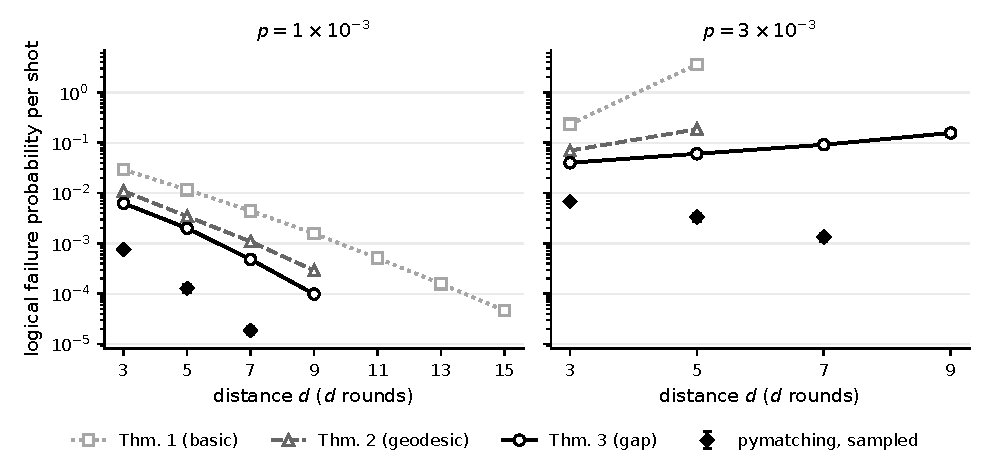
\includegraphics[width=\textwidth]{figures/bounds_vs_distance.pdf}
\caption{The three bounds and sampled pymatching rates ($99\%$ Clopper--Pearson intervals, mostly smaller than the markers) against distance for stim's rotated memory circuit with $d$ rounds. Theorem~\ref{thm:basic} is shown to $d=15$; the refinements were computed to $d=9$. Missing points are infinite bounds.}\label{fig:bounds}
\end{figure}

Table~\ref{tab:stim} and Figure~\ref{fig:bounds} give the three bounds for $d\le9$. Table~\ref{tab:basic15} gives Theorem~\ref{thm:basic} to $d=15$, including phenomenological noise.

\paragraph{Tightness.} At $p=10^{-3}$, Theorem~\ref{thm:basic} is $38$, $91$ and $240$ times the sampled rate at $d=3,5,7$, Theorem~\ref{thm:geodesic} is $14$ (at $d=3$), and Theorem~\ref{thm:gap} is $8$, $16$ and $26$ times. At $p=3\times10^{-3}$ the ratios of Theorem~\ref{thm:gap} are $6$, $18$ and $69$ at $d=3,5,7$; those of Theorem~\ref{thm:geodesic} are $10$ and $59$ at $d=3,5$, and those of Theorem~\ref{thm:basic} $35$ and $1100$. The gain of the refinements grows with $d$: at $p=10^{-3}$, Theorem~\ref{thm:geodesic} is $2.7$, $3.4$, $4.1$ and $5.4$ times below Theorem~\ref{thm:basic} at $d=3,5,7,9$, and Theorem~\ref{thm:gap} a further $1.7$--$2.9$ times. The ratio to the sampled rate still grows with $d$ for all three bounds. The looseness comes from the Peierls step (the sum over subsets of a cycle with a Chernoff factor), not from the counting of cycles: at $d=3$ with two rounds the non-backtracking walk sum exceeds the exact sum over the $29{,}138$ odd simple paths by $3\%$ (check N3 below).

\begin{table}[!htb]
\centering\small\setlength{\tabcolsep}{3.5pt}
\begin{tabular}{lccccccc}
\toprule
& $d=3$ & $5$ & $7$ & $9$ & $11$ & $13$ & $15$\\
\midrule
circuit, $10^{-4}$ & $6.8{\times}10^{-4}$ & $1.5{\times}10^{-5}$ & $2.8{\times}10^{-7}$ & $4.8{\times}10^{-9}$ & $7.4{\times}10^{-11}$ & $1.1{\times}10^{-12}$ & $1.5{\times}10^{-14}$\\
circuit, $5{\times}10^{-4}$ & $9.0{\times}10^{-3}$ & $1.3{\times}10^{-3}$ & $1.8{\times}10^{-4}$ & $2.1{\times}10^{-5}$ & $2.3{\times}10^{-6}$ & $2.4{\times}10^{-7}$ & $2.3{\times}10^{-8}$\\
circuit, $10^{-3}$ & $2.9{\times}10^{-2}$ & $1.2{\times}10^{-2}$ & $4.4{\times}10^{-3}$ & $1.6{\times}10^{-3}$ & $5.1{\times}10^{-4}$ & $1.6{\times}10^{-4}$ & $4.6{\times}10^{-5}$\\
circuit, $1.5{\times}10^{-3}$ & $6.0{\times}10^{-2}$ & $4.9{\times}10^{-2}$ & $4.4{\times}10^{-2}$ & $4.1{\times}10^{-2}$ & $3.7{\times}10^{-2}$ & $3.4{\times}10^{-2}$ & $3.0{\times}10^{-2}$\\
circuit, $2{\times}10^{-3}$ & $0.10$ & $0.16$ & $0.47$ & $\infty$ & $\infty$ & $\infty$ & $\infty$\\
phenom., $5{\times}10^{-3}$ & $5.4{\times}10^{-2}$ & $1.2{\times}10^{-2}$ & $2.1{\times}10^{-3}$ & $3.5{\times}10^{-4}$ & $5.3{\times}10^{-5}$ & $7.5{\times}10^{-6}$ & $1.0{\times}10^{-6}$\\
\quad sampled & $2.2{\times}10^{-3}$ & $3.2{\times}10^{-4}$ & & & & & \\
phenom., $10^{-2}$ & $0.18$ & $0.11$ & $6.0{\times}10^{-2}$ & $3.1{\times}10^{-2}$ & $1.5{\times}10^{-2}$ & $6.8{\times}10^{-3}$ & $3.0{\times}10^{-3}$\\
\quad sampled & & $2.5{\times}10^{-3}$ & $5.9{\times}10^{-4}$ & & & & \\
\bottomrule
\end{tabular}
\caption{Theorem~\ref{thm:basic} for stim's rotated memory circuit with $d$ rounds, for $3\le d\le15$, under uniform circuit noise and phenomenological noise (strength in the first column), minimized over $\lambda$. Sampled pymatching rates for circuit noise are in Table~\ref{tab:stim}.}\label{tab:basic15}
\end{table}

\paragraph{Range of validity.} A bound is finite when its walk sum converges. The largest $p$ with a finite bound is, at $d=5,7,9$: $3.2$, $2.3$, $2.0\times10^{-3}$ for Theorem~\ref{thm:basic}; $4.5$, $3.0$, $2.5\times10^{-3}$ for Theorem~\ref{thm:geodesic}; and $6.9$, $4.4$, $3.6\times10^{-3}$ for Theorem~\ref{thm:gap}. These ranges shrink with $d$ and are far below the circuit-level threshold of matching (sampled rates still decrease with $d$ at $p=3\times10^{-3}$, Table~\ref{tab:stim}). A finite bound can also exceed $1$.

\paragraph{Every-$d$ statements.} Table~\ref{tab:lattice} lists the certified exponents. Proposition~\ref{prop:lattice} gives $\Lambda^\ast=86$, $39$, $12.0$, $3.83$ at $p=10^{-4}$, $2\times10^{-4}$, $5\times10^{-4}$, $10^{-3}$, and a positive exponent for $p<1.405\times10^{-3}$ (the bulk growth rate alone reaches $1$ at $p=1.55\times10^{-3}$). Proposition~\ref{prop:lattice-gap} with $L=16$ gives $\Lambda^\ast\ge3.97$ at $p=10^{-3}$ and a positive exponent for $p<1.556\times10^{-3}$, but a slightly smaller exponent than Proposition~\ref{prop:lattice} at $p=5\times10^{-4}$; both hold, so the better one applies at each $p$. The sampled suppression factor at $p=10^{-3}$ is $\Lambda\approx6.0$ ($d=3\to5$) and $6.9$ ($d=5\to7$). The closed-form every-$d$ bounds are much weaker than the finite-$d$ evaluations at moderate $d$: at $p=10^{-3}$, Proposition~\ref{prop:lattice} gives $1.26$, $0.51$ and $4.3\times10^{-2}$ at $d=5$, $9$, $15$ (optimized over $\theta$), against $4.6\times10^{-5}$ from Theorem~\ref{thm:basic} evaluated at $d=15$; Proposition~\ref{prop:lattice-gap} gives $0.88$ at $d=9$, $6.1\times10^{-2}$ at $d=15$ and $4.0\times10^{-4}$ at $d=25$ on a grid of $\theta$. Their value is the exponent, not the prefactor. The gain of Proposition~\ref{prop:lattice-gap} over Proposition~\ref{prop:lattice} is small compared with the gain of Theorem~\ref{thm:gap} at finite $d$, for two reasons: the per-offset weights vary by up to about $13\%$ between bulk and boundary rows, so the Chernoff form of the geodesic constraint admits many non-geodesic paths, and junction constraints are dropped between blocks.

\begin{table}[!htb]
\centering\small
\begin{tabular}{lcccc}
\toprule
noise, $p$ & $\theta^\ast$ (Prop.~\ref{prop:lattice}) & $\Lambda^\ast$ & $\theta^\ast$ (Prop.~\ref{prop:lattice-gap}) & $\Lambda^\ast$\\
\midrule
circuit, $10^{-4}$ & $2.23$ & $86$ & & \\
circuit, $2\times10^{-4}$ & $1.83$ & $39$ & & \\
circuit, $5\times10^{-4}$ & $1.24$ & $12.0$ & $\ge1.195$ & $\ge10.9$\\
circuit, $10^{-3}$ & $0.671$ & $3.83$ & $\ge0.690$ & $\ge3.97$\\
circuit, $1.5\times10^{-3}$ & $0$ & -- & $\ge0.188$ & $\ge1.46$\\
phenom., $10^{-3}$ & $1.93$ & $48$ & & \\
phenom., $2\times10^{-3}$ & $1.53$ & $21$ & & \\
phenom., $5\times10^{-3}$ & $0.915$ & $6.2$ & & \\
\midrule
range ($\theta^\ast>0$) & \multicolumn{2}{c}{$p<1.405\times10^{-3}$ (phenom.\ $<1.01\times10^{-2}$)} & \multicolumn{2}{c}{$p<1.556\times10^{-3}$}\\
\bottomrule
\end{tabular}
\caption{Certified suppression exponents $\theta^\ast$ and factors $\Lambda^\ast=e^{2\theta^\ast}$ for stim's rotated memory circuit with $d$ rounds. Proved for $5\le d\le15$; for larger $d$ conditional on (H1)--(H2) and, for Proposition~\ref{prop:lattice-gap}, (A1)--(A2). The values for Proposition~\ref{prop:lattice-gap} are lower bounds from a bisection in $\theta$ at fixed $(\lambda,\mu)$. Proposition~\ref{prop:lattice-gap} was not evaluated for phenomenological noise.}\label{tab:lattice}
\end{table}

\subsection{Checks}\label{sec:checks}

Every proof step that a computation can test was tested on sampled faults or by exact enumeration on small models.
\begin{itemize}[leftmargin=*,itemsep=1pt]
\item[N1] Structure: flag consistency, balance, and one edge per mechanism after re-decomposition, for circuit and phenomenological noise at $d=3,5,7$ (and for $d\le15$ in the main computation).
\item[N2] Lemma~\ref{lem:cycle} with pymatching on sampled faults ($d=3,5$, $p=6\times10^{-3}$, $106$ failures): every failure has an odd cycle in $X\oplus\Co$, and every cycle satisfies the minimality inequality with slack at most $\delta|\gamma|$ (the largest excess found is $10^{-16}$, floating-point error).
\item[N3] The Chernoff step and the walk sum by exact enumeration at $d=3$: the sum over the $29{,}138$ odd simple paths is $0.0669$, the walk sum $0.0689$.
\item[N4] Theorem~\ref{thm:basic} lies above the $99\%$ lower limit of the sampled rate at five points (circuit and phenomenological noise).
\item[N5] Proposition~\ref{prop:lattice}: the envelope is independent of $d$ and the closed form dominates the walk sum at $d=5,7,9$.
\item[G1] Lemma~\ref{lem:geodesic}: on sampled failures ($d=3,5$, $p\in\{6\times10^{-3},10^{-2}\}$, $291$ failures) all $752$ correction runs are geodesics of pymatching's integer weights.
\item[G2] Theorem~\ref{thm:geodesic}: exact enumeration of odd simple cycles and admissible subsets on three small models (repetition code $d=3$ with $2$ rounds and $d=5$ with $1$ round; surface code $d=3$ with one round): the computable form exceeds the restricted sum by a factor $1.3$--$2.4$, and the restricted sum is $1.7$--$19$ times below Theorem~\ref{thm:basic}(a).
\item[G3] Theorem~\ref{thm:geodesic} lies above the sampled rate ($d=3,5$).
\item[G4] Lemma~\ref{lem:gap} holds on all $1{,}115$ cycles of $X\oplus\Co$ from sampled faults.
\item[G5] Theorem~\ref{thm:gap}(b) on four small models, one at circuit level with $581$ odd cycles: exact restricted sum $\le$ computable form $\le$ the same form without the junction constraint, at three values of $\lambda$.
\item[G6] Theorem~\ref{thm:gap} lies above the sampled rate at $d=3,5,7$.
\end{itemize}
No check failed. Checks of this kind can find errors in the implementation or the argument but do not replace a proof; the computations themselves are in floating point.

\subsection{Hardware error models: the certifiability margin}

Google published, with the data of the Sycamore~\cite{Google22} and Willow~\cite{Google24} surface-code experiments, the detector error models used by their decoders~\cite{ZenodoSycamore,ZenodoWillow}. All of them pass the structural checks (flag consistency, balance, exclusivity after re-decomposition). We evaluate the bounds for pymatching with the weights of these models. For Willow we use the models with the RL-optimized prior of the correlated-matching decoder, which is fitted to the data, and, for comparison, the SI1000 prior; for Sycamore we use the two models estimated from the data by the $p_{ij}$ method (\tsc{pij\_from\_even\_for\_odd}, \tsc{pij\_from\_odd\_for\_even}).

These bounds are statements about the model, not about the device: if the device were exactly described by the model, pymatching with the model's weights would fail with at most the stated probability. To summarize how far the models are from the region where the bounds work, we define the \emph{certifiability margin} $s^\ast$: the largest factor $s\le4$ such that the model with every mechanism probability $p_m$ replaced by $\min(\tfrac12,sp_m)$ (and pymatching's weights rebuilt) has a finite bound. $s^\ast>1$ means that the bound is finite at the model's own noise; it does not mean that its value is small. For Theorem~\ref{thm:basic}, $s^\ast$ is computed at $\lambda=\tfrac12$; for Theorems~\ref{thm:geodesic} and~\ref{thm:gap} on $\lambda$ grids. Bisection is to relative precision $10^{-3}$ (Theorem~\ref{thm:basic}) and $10^{-2}$ (Theorems~\ref{thm:geodesic},~\ref{thm:gap}).

\begin{table}[!htb]
\centering\small\setlength{\tabcolsep}{5pt}
\begin{tabular}{llccc}
\toprule
device, model & $d$ (experiments) & Thm.~\ref{thm:basic} & Thm.~\ref{thm:geodesic} & Thm.~\ref{thm:gap}\\
\midrule
Willow, RL prior, $10$ rounds & $3$ ($18$) & $1.29$ $[0.99,1.65]$ & $2.30$ $[1.59,3.12]$ & $3.88$ $[2.67,\,{\ge}4]$\\
 & $5$ ($8$) & $0.49$ $[0.47,0.53]$ & $0.74$ $[0.69,0.79]$ & $1.11$ $[1.04,1.19]$\\
 & $7$ ($2$) & $0.38$ $[0.38,0.38]$ & $0.55$ $[0.54,0.55]$ & $0.79$ $[0.79,0.80]$\\
\midrule
Willow, SI1000 prior, $10$ rounds & $3$ ($18$) & $3.24$ $[3.17,3.26]$ & ${\ge}4$ & ${\ge}4$\\
 & $5$ ($8$) & $1.41$ $[1.40,1.41]$ & $1.86$ $[1.85,1.86]$ & $2.81$ $[2.80,2.81]$\\
 & $7$ ($2$) & $1.10$ $[1.10,1.10]$ & $1.38$ $[1.38,1.38]$ & $2.01$ $[2.01,2.01]$\\
\midrule
Sycamore, $p_{ij}$, ${\ge}15$ rounds & $3$ ($48$) & $0.52$ $[0.41,0.62]$ & $0.98$ $[0.70,1.15]$ & $1.63$ $[1.12,2.35]$\\
 & $5$ ($12$) & $0.19$ $[0.19,0.20]$ & $0.29$ $[0.28,0.30]$ & $0.43$ $[0.42,0.45]$\\
\bottomrule
\end{tabular}
\caption{Certifiability margin $s^\ast$ (median and range over patches, bases and, for Sycamore, round counts $15,17,\dots,25$) for pymatching on Google's published error models. For Sycamore, each experiment's value is the mean over the two $p_{ij}$ models. ${\ge}4$: the search was capped at $s=4$ (for Willow $d=3$ with the RL prior, $8$ of $18$ experiments reach the cap under Theorem~\ref{thm:gap}). The bound is finite at the model's own noise iff $s^\ast>1$.}\label{tab:hardware}
\end{table}

\begin{figure}[!htb]
\centering
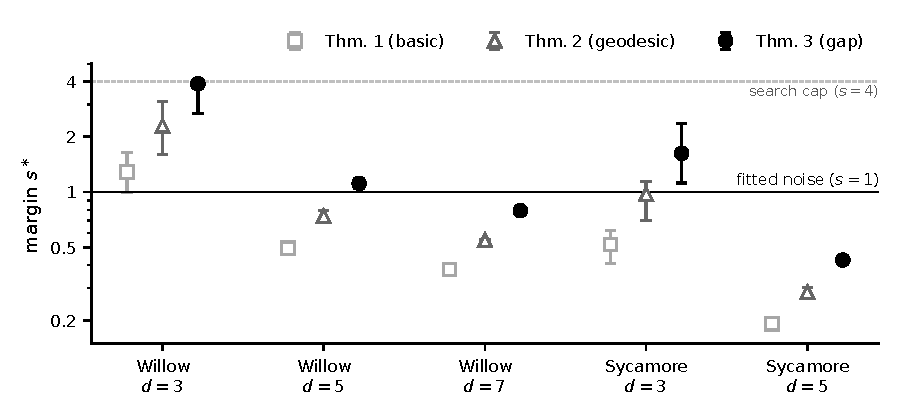
\includegraphics[width=0.85\textwidth]{figures/hardware_margins.pdf}
\caption{Certifiability margins $s^\ast$ of Table~\ref{tab:hardware} for the data-fitted models (Willow: RL prior, $10$ rounds; Sycamore: $p_{ij}$ models, $\ge15$ rounds): median and range. Above the line $s=1$ the bound is finite at the fitted noise. For Willow $d=3$, the upper end of the range of Theorem~\ref{thm:gap} is the search cap.}\label{fig:hardware}
\end{figure}

Table~\ref{tab:hardware} and Figure~\ref{fig:hardware} show the result. For the data-fitted Willow models, Theorem~\ref{thm:gap} is finite at the fitted noise at $d=3$ and, for all eight patches, at $d=5$; but at $d=5$ its value lies between $2.2$ and $10.9$, so it is vacuous. (These values were computed with the released code from the same models; they are not stored in the results file.) For comparison, the failure rates of pymatching on the $d=5$, $10$-round experiments are $0.042$--$0.060$ per shot (Table~\ref{tab:data}). At $d=7$ the bound is finite only if all fault probabilities are multiplied by $0.79$ or less. For the Willow $d=7$ patch with the SI1000 prior, at its stated noise, Theorem~\ref{thm:geodesic} gives $9.4\times10^{-2}$ and Theorem~\ref{thm:gap} $2.2\times10^{-2}$ ($Z$ basis, $10$ rounds), but that prior is not fitted to the data. For Sycamore the sharpest bound is finite at $d=3$ and requires noise about $2.3$ times lower at $d=5$. The gap between the margins of the SI1000 and the fitted Willow models shows that the fitted models are about $2.5$ times noisier in the sense relevant here. In short, the bounds do not certify the logical error rates of these devices: they certify that the fitted models at $d\le5$ lie inside the region where the walk sums converge, and they quantify by how much the noise of the $d=7$ model would have to decrease.

\subsection{Data certificates}

\paragraph{Validation on simulated data.} On $2\times10^6$ shots of stim's circuit ($d=3$, $3$ rounds, $p=2\times10^{-3}$), the identity of Proposition~\ref{prop:data-cert}(a) recovers all $55$ edge probabilities ($q_e\le9.8\times10^{-3}$) to within $1.8\times10^{-4}$. For $20$ independent data sets of $50{,}000$ shots, every edge interval covered the true $q_e$ in all $20$ sets, for all three methods and for two models (stim's circuit with $9$ rounds, and Willow's published $d=3$ model, sampled). With $20$ repetitions this is a smoke test, not a test of the confidence level. The certified bound (Theorem~\ref{thm:geodesic}, median over five data sets, paired intervals) was $0.34$ for stim's circuit, against $0.098$ at the true $q$ and a sampled pymatching rate of $8.7\times10^{-3}$; for the Willow model it was $2.1$ (true $q$: $0.57$; sampled: $0.066$). Pooling under (T) gave $0.21$ and $1.2$.

\begin{table}[!htb]
\centering\small\setlength{\tabcolsep}{4pt}
\begin{tabular}{lcccccc}
\toprule
device, $d$, rounds (n) & certified & at point est. & observed & ratio & pass\\
\midrule
Willow $3$, $1$ ($18$) & $0.051$--$0.16$ & $0.021$--$0.064$ & $0.0027$--$0.018$ & $6.5$--$24$ & $7$\\
Willow $5$, $1$ ($8$) & $0.20$--$0.41$ & $0.029$--$0.050$ & $0.0011$--$0.0033$ & $76$--$191$ & $1$\\
Willow $7$, $1$ ($2$) & $2.2$--$8.7$ & $0.022$--$0.025$ & $0.0004$--$0.0006$ & -- & $0$\\
Willow $3$, $10$ ($18$) & $1.5$--$21$ & $0.46$--$1.7$ & $0.061$--$0.13$ & -- & $9$\\
Willow $5$, $10$ ($8$) & $\infty$ & $\infty$ & $0.042$--$0.060$ & -- & $0$\\
Willow $7$, $10$ ($2$) & $\infty$ & $\infty$ & $0.027$--$0.033$ & -- & $0$\\
Sycamore $3$, $1$ ($8$) & $0.27$--$0.32$ & $0.12$--$0.13$ & $0.016$--$0.019$ & $14$--$19$ & $4$\\
Sycamore $3$, $3$ ($8$) & $4.0$--$\infty$ & $0.92$--$1.9$ & $0.080$--$0.093$ & -- & $3$\\
Sycamore $5$, $1$ ($2$) & $\infty$ & $0.49$--$0.60$ & $0.0079$--$0.0091$ & -- & $2$\\
Sycamore $5$, $3$ ($2$) & $\infty$ & $\infty$ & $0.071$--$0.079$ & -- & $0$\\
\bottomrule
\end{tabular}
\caption{Data certificates (Proposition~\ref{prop:data-cert}, Theorem~\ref{thm:geodesic}, paired intervals, $\delta=10^{-3}$, no (T)), ranges over experiments. ``At point est.'': the same bound at the point estimate of $q$. ``Observed'': pymatching with the decoder's weights on the same $50{,}000$ shots. ``Ratio'': certified over observed, where both are finite and the certificate is below $1$. ``Pass'': experiments that pass both diagnostics of (G) (no significant non-edge covariance, no significant drift). Decoder models: Willow, RL prior; Sycamore, $p_{ij}$ (even for odd).}\label{tab:data}
\end{table}

\paragraph{Hardware.} Table~\ref{tab:data} summarizes the certificates on the Willow and Sycamore data. The certificate is non-vacuous only for one-round experiments at $d\le5$, where it is $6$--$190$ times the observed pymatching rate. At $d=3$ the bound at the point estimate is already $2.7$--$8.5$ times the observed rate and the confidence limits add a factor $2.2$--$3$; at $d=5$ these factors are $10$--$28$ and $7$--$8$. Theorem~\ref{thm:basic} in place of Theorem~\ref{thm:geodesic} is $3.4$--$4.6$ times larger at $d=3$ and $16$ times larger or infinite at $d=5$. For Willow with $10$ rounds the certificates are vacuous at $d=3$ ($0.93$--$4.9$ under (T), two of $18$ below $1$) and infinite at $d=5,7$, already at the point estimate. The limits are widest at the boundary edges, where $q_b$ is determined only by a marginal $a_i$ and inherits the limits of the neighbouring edges.

\paragraph{The assumptions fail in part.} Non-edge covariances above the Bonferroni threshold occur in $8$ of the $18$ Willow $d=3$ one-round experiments and in $6$ of the $8$ at $d=5$. Most are marginal ($|z|\le6$), but one pair of final-round detectors recurs with $|z|=15$--$19$ in the $d=5$ and $d=7$ patches, and the $d=7$, $10$-round $Z$ experiment shows long-range time correlations at one plaquette, typical of leakage. Identical distribution fails as well: in some Sycamore experiments single-detector rates change by factors of $2$--$5$ between blocks of $5{,}000$--$10{,}000$ consecutive shots, and the drift statistic exceeds its threshold in $4$ of $8$ Sycamore and $4$ of $18$ Willow one-round $d=3$ experiments. The experiments that pass both diagnostics are $7$ Willow $d=3$ experiments (certified $0.065$--$0.11$ against observed $0.0034$--$0.017$) and $4$ Sycamore $d=3$ experiments ($0.27$--$0.31$ against $0.016$--$0.017$). For the others the certificate is conditional on an assumption that the data contradict. Passing the diagnostics does not prove (G).

\section{Software}\label{sec:software}

The bounds are implemented in the Python package \tsc{lcd-qec} (version 0.1.0, Apache-2.0 licence; source at \url{https://github.com/RuiZhu1/coset-distinguishability}, import name \tsc{lcd}), installed with \tsc{pip install "lcd-qec[sinter]"}. The command
\begin{center}\small
\tsc{lcd-peierls --generated surface\_code:rotated\_memory\_z -d 5 -p 1e-3}
\end{center}
prints the smallest of the three bounds for the generated circuit (here $\pM\le2.0\times10^{-3}$, Theorem~\ref{thm:gap}), the optimal $\lambda$ and the certified upper bound on the spectral radius; \tsc{lcd-peierls circuit.stim model.dem --json} does the same for user circuits and detector error models, and \tsc{--method} selects a theorem. The tool refuses models whose flags are inconsistent, whose observable graph is not balanced, or which leave non-exclusive mechanisms after re-decomposition.

\paragraph{Several observables.} For a model with $k$ observables, observable $j$ fails iff its parity on $X\oplus C$ is odd. Projecting the model onto observable $j$ leaves the graph and the decoder's weights unchanged provided no two parallel mechanisms differ only in the dropped observables; the tool checks this by comparing pymatching's weights before and after projection. Each per-observable bound then applies, and $\Prob[\text{some observable fails}]\le\sum_j B_j$, which is the event counted as an error by sinter.

\paragraph{Sinter and hardware models.} \tsc{lcd.\allowbreak integrations.\allowbreak sinter\_peierls.\allowbreak compare(tasks, stats)} attaches to every sinter task the bound, the sampled rate with its interval, their ratio, and a consistency flag (a sampled rate significantly above a bound would indicate an error). \tsc{lcd.\allowbreak integrations.\allowbreak zenodo.\allowbreak willow\_dem} fetches a single published Willow model from the Zenodo record by HTTP range requests (about $0.4$\,MB instead of the full archive), and \tsc{lcd.\allowbreak analysis.\allowbreak hardware.\allowbreak certifiability\_margin} computes $s^\ast$. Two example notebooks reproduce a sinter comparison and the Willow margin.

\section{Related work}\label{sec:related}

\paragraph{Peierls arguments and thresholds.} The Peierls argument for matching on the surface code is due to Dennis, Kitaev, Landahl and Preskill~\cite{DKLP}, who count self-avoiding paths that carry at least half their weight in errors; Remark~\ref{rem:cc} is this argument with the count made explicit. Kovalev and Pryadko~\cite{KovalevPryadko} prove that low-density parity-check code families whose distance grows as a power of the length correct errors below a positive error rate, and Dumer, Kovalev and Pryadko~\cite{DKP} give analytic threshold bounds combining erasures, depolarizing and syndrome errors. Fowler~\cite{Fowler} proved a finite threshold for matching under circuit-level noise for one fixed surface-code circuit in which every elementary operation fails with probability $p$, with the condition $p<7.4\times10^{-4}$. Theorem~\ref{thm:basic} is a bound of the same kind, but it is evaluated on a given detector error model with its own constants, and it applies to any model whose observable graph passes the balance check. A threshold for the union-find decoder under circuit-level local stochastic noise is proved in~\cite{YLY}. For concatenated codes, Aliferis, Gottesman and Preskill~\cite{AGP} proved a circuit-level threshold with explicit constants, including noise correlated in space and time, by an inductive and computer-assisted argument. For general non-Pauli noise, Chai and Ng~\cite{ChaiNg} show that extending existing proof techniques gives no nontrivial threshold for the surface code. Pryadko~\cite{Pryadko} describes the exact error distribution of a Clifford measurement circuit and maximum-likelihood decoding with it.

\paragraph{Estimates of logical error rates.} Experimental suppression factors are reported as fits with statistical error bars~\cite{Google22,Google24}. Rare-event sampling reaches small failure probabilities at fixed parameters~\cite{BV,Mayer}, and closed-form approximations count failing configurations~\cite{Regev}. These are estimates; our bounds are guarantees for a given model, at the price of looseness. Takou et al.~\cite{Takou} estimate logical error rates from the syndrome data of surface-code experiments, including Willow and IBM data.

\paragraph{Noise estimation from syndromes.} The $p_{ij}$ method~\cite{Google21} estimates edge probabilities from two-point correlations of detection events, and Spitz et al.~\cite{Spitz} estimate matching weights from pair correlators in a time-dependent environment. Wagner, Kampermann, Bru{\ss} and Kliesch give general conditions under which error rates are identifiable from syndrome statistics~\cite{WKBK21} and prove that Pauli channels with correlations up to the pure distance can be estimated from syndrome measurements of stabilizer codes~\cite{WKBK22}. Proposition~\ref{prop:data-cert} uses the simplest instance of such an identity (the graph case) and adds what is needed for a certificate: simultaneous confidence limits, their propagation to the boundary edges, and the monotonicity of the bounds in the limits.

\paragraph{Decoders not covered.} Our bounds concern minimum-weight matching with fixed weights. Correlated matching~\cite{FowlerCorr} reweights edges after a first matching pass, belief matching~\cite{BeliefMatching} sets weights shot by shot from belief propagation on the full detector error model, and the decoders used for Willow~\cite{Google24} include correlated matching with a fitted prior and neural-network decoders. For these, the minimality argument of Lemma~\ref{lem:cycle} does not hold with fixed weights, and our bounds do not apply; by Lemma~\ref{lem:bayes} they still bound the maximum-likelihood failure probability, which these decoders approximate.

\paragraph{Bursts.} Error bursts and the floor they impose are studied experimentally~\cite{McEwen,Google22,Google24}, and the resilience of the surface code to bursts is studied by simulation in~\cite{TPMP}. Proposition~\ref{prop:bursts} is a bound of a different kind, for a stochastic burst model with bounded region size and rate, uniform in the burst strength.

\section{Limitations and outlook}\label{sec:limits}

\begin{enumerate}[leftmargin=*,itemsep=2pt]
\item \emph{Looseness.} The sharpest bound is $6$--$69$ times the sampled pymatching rate at the points tested, and the ratio grows with $d$ and $p$. The certified $\Lambda^\ast\ge3.97$ at $p=10^{-3}$ compares with a sampled $\Lambda\approx6$--$7$. The loss sits in the Peierls step; the refinements recover part of it.
\item \emph{Hardware.} On data-fitted Willow models the bound is finite at $d=3$ and $5$ but vacuous at $d=5$ ($2.2$--$10.9$), and the $d=7$ model is outside the range of convergence ($s^\ast=0.79$). The certified suppression factor concerns stim's uniform noise model and says nothing about a device. Statements about a device additionally need a model of the device that is itself certified; the data certificate is a first attempt.
\item \emph{Data certificate.} It is non-vacuous only for one-round experiments at $d\le5$ and is conditional on (G), which fails in part of the data (non-edge correlations, drift, leakage-like time correlations). Joint confidence regions for $(a_i,T_{ij})$, a boundary statistic that cancels the neighbouring edges to first order, and a version of (G) with hyperedges are natural next steps.
\item \emph{Every $d$.} The hypotheses (H1)--(H2), (A1)--(A2) are checked for $d\le15$ ($d\le13$ for the envelopes in (A1)) and are conditional beyond; a proof from the structure of the generated circuit is missing.
\item \emph{Computer assistance.} All bounds are computed in floating point (sparse LU factorizations, eigenvalue computations for the lattice matrices), without interval arithmetic. The convergence certificate (positive solution of $(I-B)z=\one$) is also evaluated in floating point.
\item \emph{Scope.} Minimum-weight matching only, with weights fixed before the shot; one or several observables via a union bound; detector error models with a balanced observable graph and exclusive mechanisms after re-decomposition. Erasure flags at circuit level (weights that change shot by shot), non-balanced models, and models with non-exclusive mechanisms (to which Theorem~\ref{thm:basic}(a) applies via the splitting factor, but which we have not computed) are not covered. Only surface-code memory experiments were evaluated.
\end{enumerate}

\paragraph{Note on the status of the proofs.} The proofs in this paper are complete as written but are drafts that have not been independently reviewed. The numerical checks of Section~\ref{sec:checks} test their steps on examples.

\section*{Acknowledgments}
[Acknowledgments.] We thank Google Quantum AI for publishing the data and decoder models of~\cite{Google22,Google24}.

\appendix

\section{Reproducibility}\label{app:repro}

All results are produced by scripts in the repository of Section~\ref{sec:software}; every results file records the script, the git commit and whether the source tree was clean (\tsc{git\_dirty\_src}). The hardware data are not part of the repository; they are the Zenodo records~\cite{ZenodoSycamore,ZenodoWillow} (for Willow, a partial extraction of the $d=3,5,7$ patches). The figures of this paper are produced by \tsc{papers\sla circuit-bounds\sla figures\sla make\_figures.py} from the results files, which also prints the numbers of Tables~\ref{tab:hardware} and~\ref{tab:data}.

\begin{table}[h]
\centering\footnotesize\setlength{\tabcolsep}{3pt}
\begin{tabular}{>{\raggedright}p{3.6cm}>{\raggedright}p{2.0cm}>{\raggedright}p{6.2cm}p{2.0cm}}
\toprule
This paper & Notes & Script $\to$ results file & Commit\\
\midrule
Def.~\ref{def:obs-graph}, Lemma~\ref{lem:cycle}, Thm.~\ref{thm:basic}, Prop.~\ref{prop:bursts} & Def.~4.27, Thm.~4.28 & \tsc{experiments\sla certification\sla circuit\_peierls.py} $\to$ \tsc{circuit\_peierls.json} & \tsc{1ea2748}\\
Lemma~\ref{lem:bayes} & Lemma~1.4 & -- & --\\
Remark~\ref{rem:cc} & Thm.~4.15 & -- & --\\
Prop.~\ref{prop:lattice}, Table~\ref{tab:lattice} & Props.~4.29, 4.30 & same & \tsc{1ea2748}\\
Checks N1--N5 & \S4.9 & \tsc{theory\sla checks\sla circuit\_peierls\_checks.py} $\to$ \tsc{circuit\_peierls\_checks.json} & file at \tsc{a8c3b7f}$^\ast$\\
Lemma~\ref{lem:geodesic}, Thm.~\ref{thm:geodesic} & Thm.~4.32 & \tsc{experiments\sla certification\sla circuit\_peierls\_geodesic.py} $\to$ \tsc{circuit\_peierls\_geodesic.json} & \tsc{77567ef}\\
Lemma~\ref{lem:gap}, Thm.~\ref{thm:gap} & Thm.~4.34 & same & \tsc{77567ef}\\
Checks G1--G6 & \S4.9 & \tsc{theory\sla checks\sla geodesic\_checks.py} $\to$ \tsc{geodesic\_checks.json} & file at \tsc{6a6f5ad}$^\ast$\\
Prop.~\ref{prop:lattice-gap} & Prop.~4.35 & \tsc{experiments\sla certification\sla lattice\_gap.py} $\to$ \tsc{lattice\_gap.json} & \tsc{799463c}\\
Prop.~\ref{prop:data-cert}, Table~\ref{tab:data} & Prop.~4.33 & \tsc{experiments\sla hardware\sla data\_certificate.py} $\to$ \tsc{data\_certificate.json} & \tsc{86c4ea2}\\
Table~\ref{tab:hardware}, Fig.~\ref{fig:hardware} & \S4.9 & \tsc{experiments\sla hardware\sla certifiability\_gap.py} $\to$ \tsc{hardware\_gap.json} & \tsc{6a6f5ad}\\
\bottomrule
\end{tabular}
\caption{Map from the results of this paper to the theory notes (\tsc{theory/main.tex}) and to the scripts, results files (in \tsc{results/}) and the commits recorded in them. $^\ast$These two check files do not record a commit; the commit given is the last one that changed the file.}
\end{table}

\paragraph{Computational details.} Theorem~\ref{thm:basic} is minimized over $\lambda$ by a one-dimensional search (log-convexity), Theorems~\ref{thm:geodesic} and~\ref{thm:gap} on grids of $\lambda$; geodesics are computed with the integer weights of pymatching, so equality tests in $K_C$ are exact. The data certificate uses $\lambda\in[0.05,0.5]$ on a grid of ten values. The Willow $d=5$ values of Theorem~\ref{thm:gap} at the fitted noise quoted in the text were computed with \tsc{lcd.\allowbreak analysis.\allowbreak hardware.\allowbreak bound\_at\_scale} at $s=1$ on the eight RL-prior models ($10$ rounds); they range from $2.18$ to $10.9$. Simulations of Table~\ref{tab:stim} use between $6\times10^4$ and $10^7$ shots per point; the rates at $p=3\times10^{-3}$, $d=5,7$ are from sinter runs of check G3, the others from the main computation.

\begin{thebibliography}{99}
\bibitem{DKLP} E.~Dennis, A.~Kitaev, A.~Landahl, J.~Preskill, \emph{Topological quantum memory}, J.\ Math.\ Phys.\ 43, 4452 (2002).
\bibitem{Fowler} A.~G.~Fowler, \emph{Proof of finite surface code threshold for matching}, Phys.\ Rev.\ Lett.\ 109, 180502 (2012).
\bibitem{stim} C.~Gidney, \emph{Stim: a fast stabilizer circuit simulator}, Quantum 5, 497 (2021).
\bibitem{SB} O.~Higgott, C.~Gidney, \emph{Sparse Blossom: correcting a million errors per core second with minimum-weight matching}, arXiv:2303.15933 (2023); Quantum 9, 1600 (2025).
\bibitem{BV} S.~Bravyi, A.~Vargo, \emph{Simulation of rare events in quantum error correction}, Phys.\ Rev.\ A 88, 062308 (2013).
\bibitem{IyerPoulin} P.~Iyer, D.~Poulin, \emph{Hardness of decoding quantum stabilizer codes}, IEEE Trans.\ Inf.\ Theory 61, 5209 (2015), arXiv:1310.3235.
\bibitem{DKP} I.~Dumer, A.~A.~Kovalev, L.~P.~Pryadko, \emph{Thresholds for correcting errors, erasures, and faulty syndrome measurements in degenerate quantum codes}, Phys.\ Rev.\ Lett.\ 115, 050502 (2015), arXiv:1412.6172.
\bibitem{KovalevPryadko} A.~A.~Kovalev, L.~P.~Pryadko, \emph{Fault tolerance of ``bad'' quantum low-density parity check codes}, Phys.\ Rev.\ A 87, 020304(R) (2013), arXiv:1208.2317.
\bibitem{YLY} S.~Yoshida, E.~Lake, H.~Yamasaki, \emph{Proof of a finite threshold for the union-find decoder}, arXiv:2602.20238 (2026).
\bibitem{ChaiNg} J.~H.~Chai, H.~K.~Ng, \emph{On the fault-tolerance threshold for surface codes with general noise}, arXiv:2207.00217 (2022).
\bibitem{Google22} R.~Acharya et al.\ (Google Quantum AI), \emph{Suppressing quantum errors by scaling a surface code logical qubit}, Nature 614, 676 (2023), arXiv:2207.06431.
\bibitem{Google24} R.~Acharya et al.\ (Google Quantum AI), \emph{Quantum error correction below the surface code threshold}, Nature 638, 920 (2025), arXiv:2408.13687.
\bibitem{Takou} E.~Takou, C.~Benito, A.~Vezvaee, D.~A.~Lidar, K.~R.~Brown, \emph{Logical error estimation from syndrome data of surface-code experiments}, arXiv:2606.11496 (2026).
\bibitem{Mayer} C.~Mayer, A.~Ganti, U.~Onunkwo, T.~Metodi, B.~Anker, J.~Skryzalin, \emph{Rare event simulation of quantum error-correcting circuits}, arXiv:2509.13678 (2025).
\bibitem{Regev} S.~Regev, D.~Dilley, R.~Bennink, \emph{Closed form logical error rate approximations for surface codes}, arXiv:2605.03054 (2026).
\bibitem{McEwen} M.~McEwen et al., \emph{Resolving catastrophic error bursts from cosmic rays in large arrays of superconducting qubits}, Nat.\ Phys.\ 18, 107 (2022), arXiv:2104.05219.
\bibitem{TPMP} S.~J.~S.~Tan, C.~A.~Pattison, M.~McEwen, J.~Preskill, \emph{Resilience of the surface code to error bursts}, Phys.\ Rev.\ A 113, 022450 (2026), arXiv:2406.18897.
\bibitem{Pryadko} L.~P.~Pryadko, \emph{On maximum-likelihood decoding with circuit-level errors}, Quantum 4, 304 (2020), arXiv:1909.06732.
\bibitem{AGP} P.~Aliferis, D.~Gottesman, J.~Preskill, \emph{Quantum accuracy threshold for concatenated distance-3 codes}, Quantum Inf.\ Comput.\ 6, 97 (2006), arXiv:quant-ph/0504218.
\bibitem{Spitz} S.~T.~Spitz, B.~Tarasinski, C.~W.~J.~Beenakker, T.~E.~O'Brien, \emph{Adaptive weight estimator for quantum error correction in a time-dependent environment}, Adv.\ Quantum Technol.\ 1, 1800012 (2018), arXiv:1712.02360.
\bibitem{Google21} Z.~Chen et al.\ (Google Quantum AI), \emph{Exponential suppression of bit or phase errors with cyclic error correction}, Nature 595, 383 (2021), arXiv:2102.06132.
\bibitem{WKBK21} T.~Wagner, H.~Kampermann, D.~Bru{\ss}, M.~Kliesch, \emph{Optimal noise estimation from syndrome statistics of quantum codes}, Phys.\ Rev.\ Research 3, 013292 (2021), arXiv:2010.02243.
\bibitem{WKBK22} T.~Wagner, H.~Kampermann, D.~Bru{\ss}, M.~Kliesch, \emph{Pauli channels can be estimated from syndrome measurements in quantum error correction}, Quantum 6, 809 (2022), arXiv:2107.14252.
\bibitem{BeliefMatching} O.~Higgott, T.~C.~Bohdanowicz, A.~Kubica, S.~T.~Flammia, E.~T.~Campbell, \emph{Improved decoding of circuit noise and fragile boundaries of tailored surface codes}, Phys.\ Rev.\ X 13, 031007 (2023), arXiv:2203.04948.
\bibitem{FowlerCorr} A.~G.~Fowler, \emph{Optimal complexity correction of correlated errors in the surface code}, arXiv:1310.0863 (2013).
\bibitem{WaudbySmithRamdas} I.~Waudby-Smith, A.~Ramdas, \emph{Estimating means of bounded random variables by betting}, J.\ R.\ Stat.\ Soc.\ Ser.\ B Stat.\ Methodol.\ 86, 1--27 (2024), arXiv:2010.09686.
\bibitem{ClopperPearson} C.~J.~Clopper, E.~S.~Pearson, \emph{The use of confidence or fiducial limits illustrated in the case of the binomial}, Biometrika 26, 404--413 (1934).
\bibitem{HornJohnson} R.~A.~Horn, C.~R.~Johnson, \emph{Matrix Analysis}, 2nd ed., Cambridge University Press (2012), doi:10.1017/CBO9781139020411.
\bibitem{ZenodoSycamore} Google Quantum AI, \emph{Data for ``Suppressing quantum errors by scaling a surface code logical qubit''}, Zenodo (2022), doi:10.5281/zenodo.6804040.
\bibitem{ZenodoWillow} Google Quantum AI, \emph{Data for ``Quantum error correction below the surface code threshold''}, Zenodo (2024), doi:10.5281/zenodo.13273331.
\end{thebibliography}

\end{document}
